%--------------------------------------------------
% CPSC 202: Mathematical Tools for Computer Science
% Yale University
%
% Template for Homework Assignments
% by Yiding Hao
%--------------------------------------------------
\documentclass{cpsc202}

% Please put your information here.
\myname{Chura Quispe, Victor Miguel}
\myprofessor{Marc Masias}
\mysources{Your Sources}
\hwnumber{0}
\lstset{basicstyle=\ttfamily}

% \singlesided % Uncomment to print single-sided.
\graphicspath{{./media/}}
% Start typing your solution here.
\begin{document}

    \centerline{\Large\textbf{Deep Learning Project 2: Object detection}}

    Objective of the document: Details about the process of implementing algorithms for object detection.

    \large\textbf{Part I: Inference on test images and videos.}

    Overall the problem that I chose to solve is to detect butterflies.
    Firstly because in the search of datasets to images I've found this challenge: `Butterfly Detection' by Nuwe.io.
    But the challenge is actually classification, with the intention to practice even more I attempt the challenge with the knowledge learnt from the previous Project 1.
    \begin{center}
        
\includegraphics[width=0.6\textwidth]{challenge_butterfly_classification}
        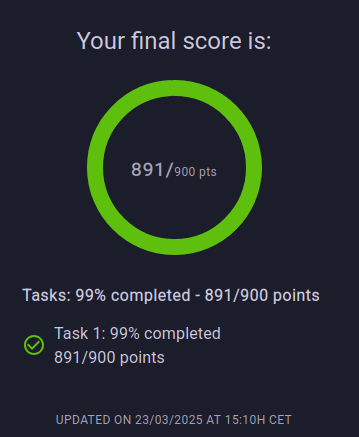
\includegraphics[width=0.3\textwidth]{challenge_result}
    \end{center}

    Back to this Project of Object Detection, I tried to use Yolo-11s on the images from the challenge I mentioned and a YouTube's video entirely of butterflies,
    the results are shown in the figure~\ref{fig:pre-trained}
    \begin{figure}
        \begin{subfigure}{.9\textwidth}
            \centering
            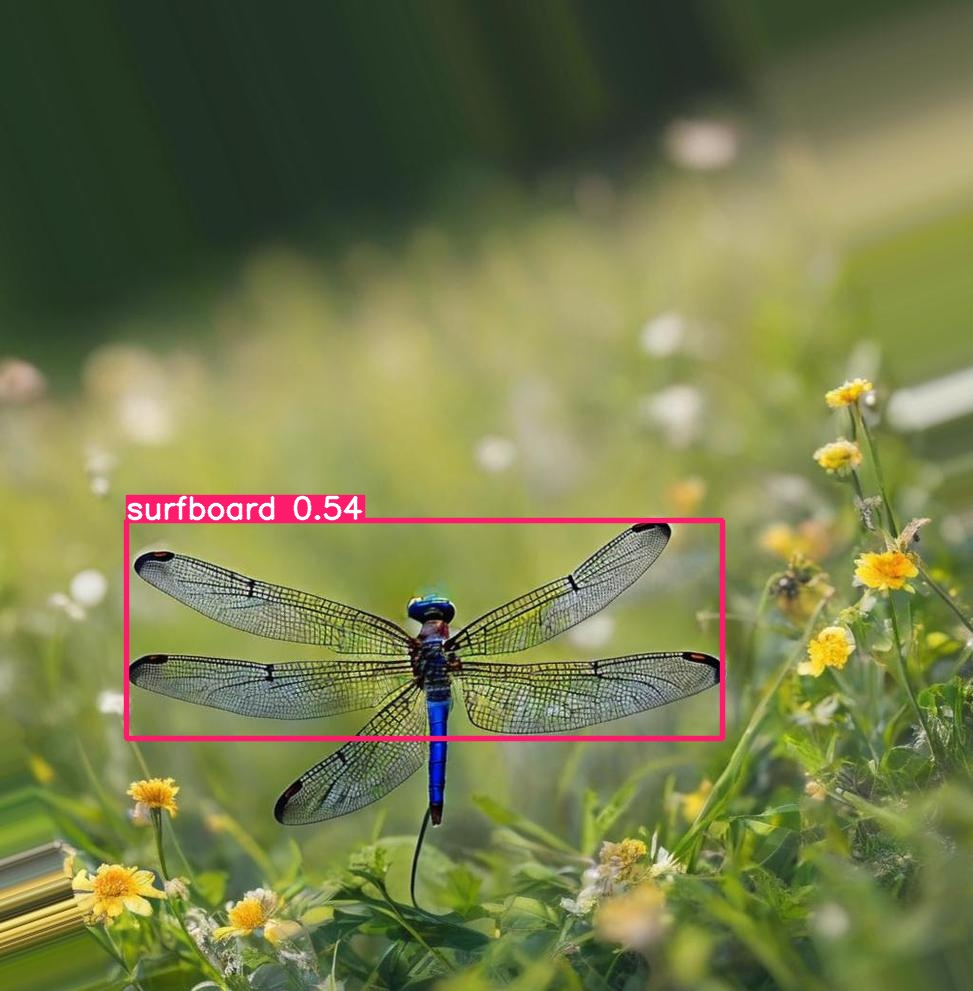
\includegraphics[width=.4\linewidth]{pretrained/negative_imagen_723}
            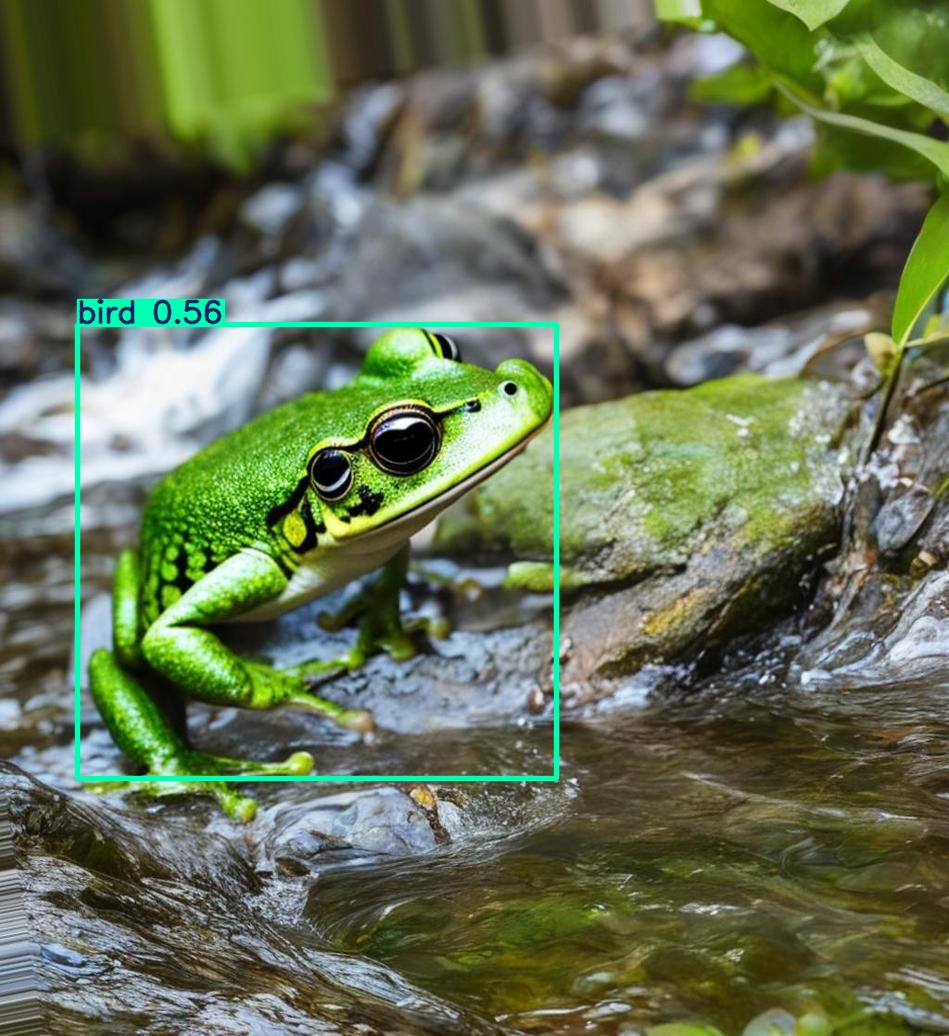
\includegraphics[width=.4\linewidth]{pretrained/negative_imagen_880}
            \caption{Negative class in the training data of the challenge}
            \label{fig:negative-pretrained}
        \end{subfigure}

        \begin{subfigure}{.9\textwidth}
            \centering
            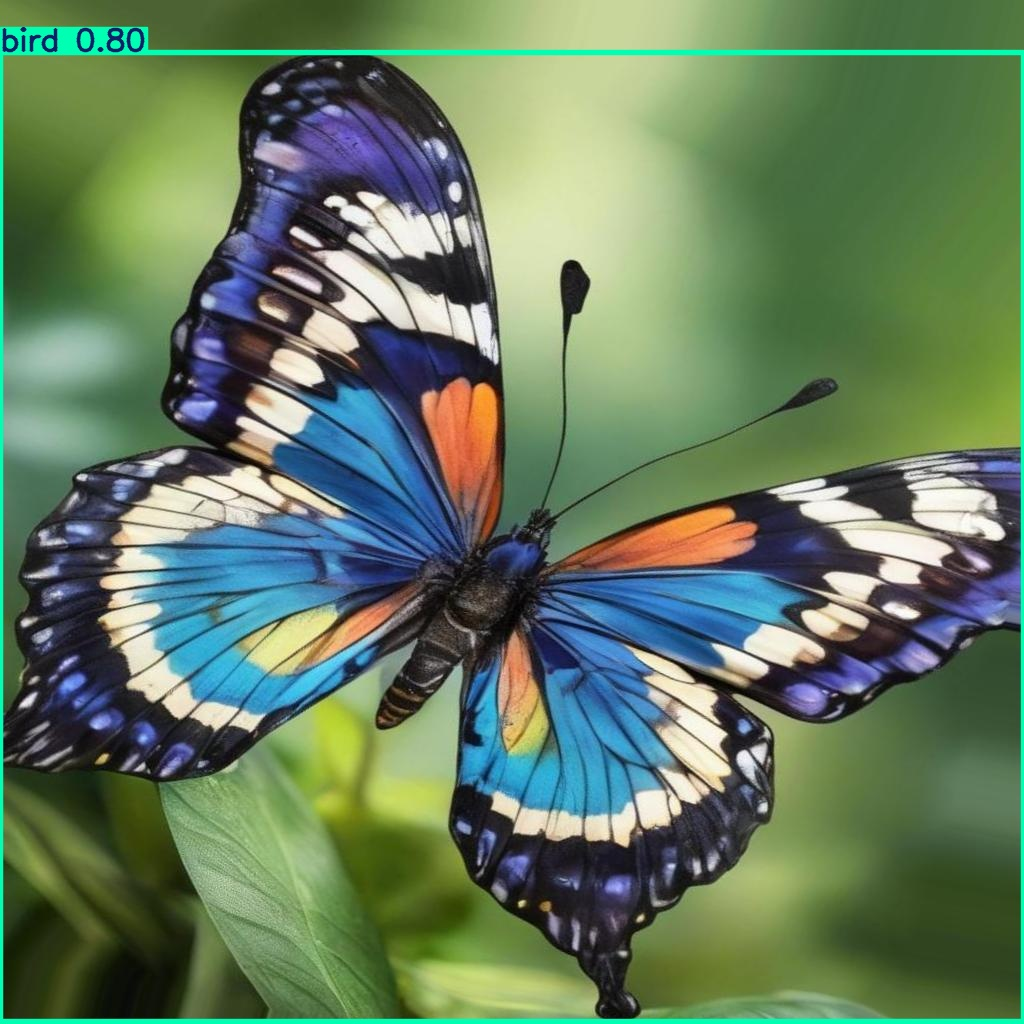
\includegraphics[width=.4\linewidth]{pretrained/positive_imagen_45}
            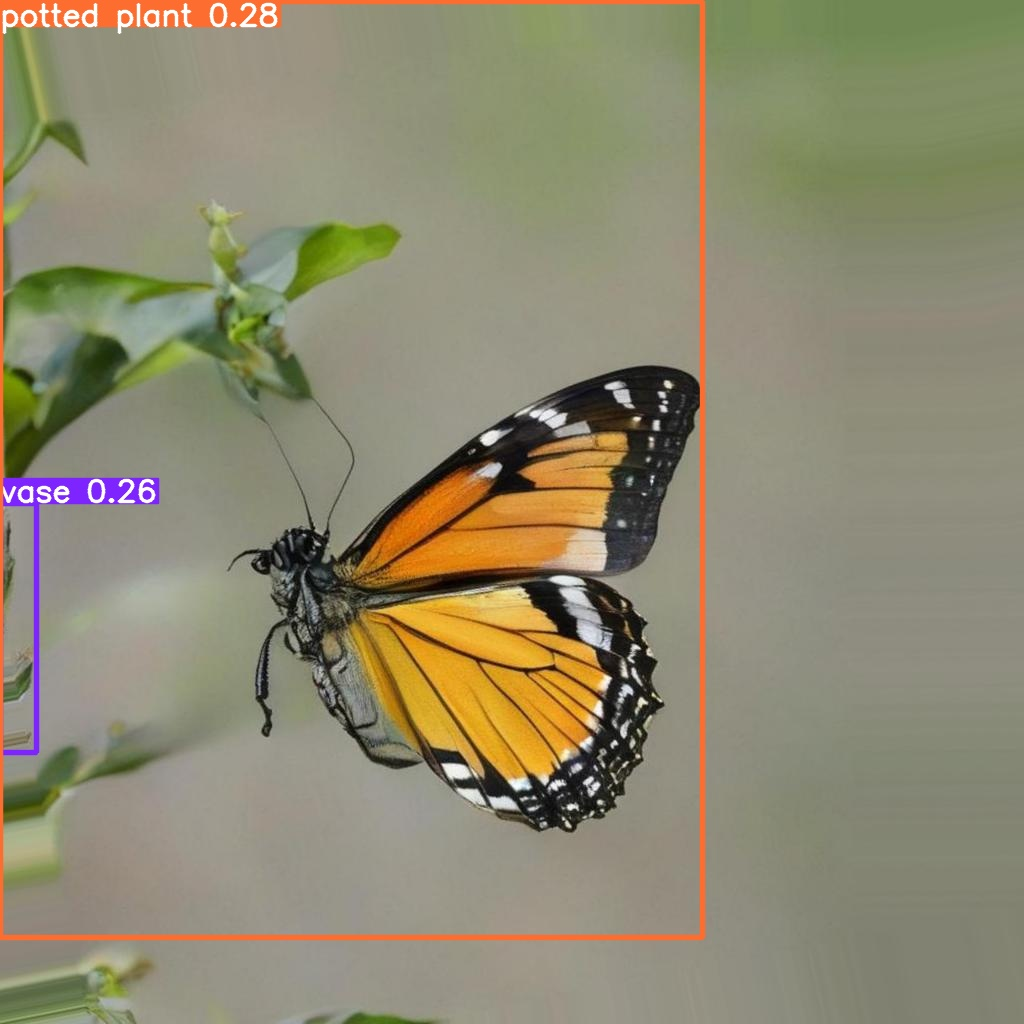
\includegraphics[width=.4\linewidth]{pretrained/positive_imagen_888}
            \caption{Positive class in the training data of the challenge}
            \label{fig:positive-pretrainied}
        \end{subfigure}

        \begin{subfigure}{.9\textwidth}
            \centering
            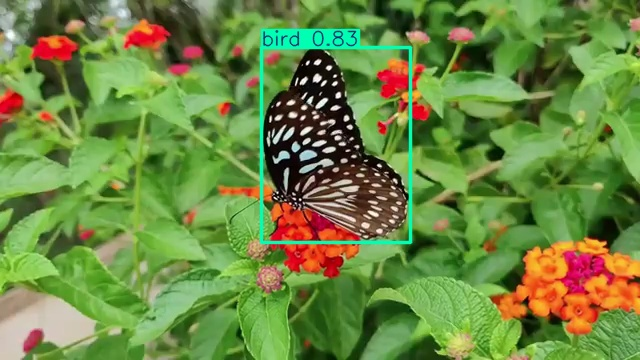
\includegraphics[width=.4\linewidth]{pretrained/photogram_16}
            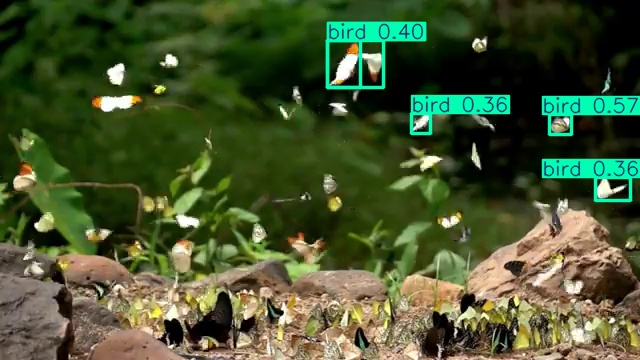
\includegraphics[width=.4\linewidth]{pretrained/photogram_93}
            \caption{Images of the YouTube video}
            \label{fig:video-pretrainied}
        \end{subfigure}
        \caption{Images results using only the pre-trained Yolo 11s}
        \label{fig:pre-trained}
    \end{figure}

    \newpage
    \large\textbf{Part II: Transfer learning to detect one novel class}
    Following the same problem, to detect butterflies, firstly I've chosen the dataset with only 2096 images.
    \begin{center}
        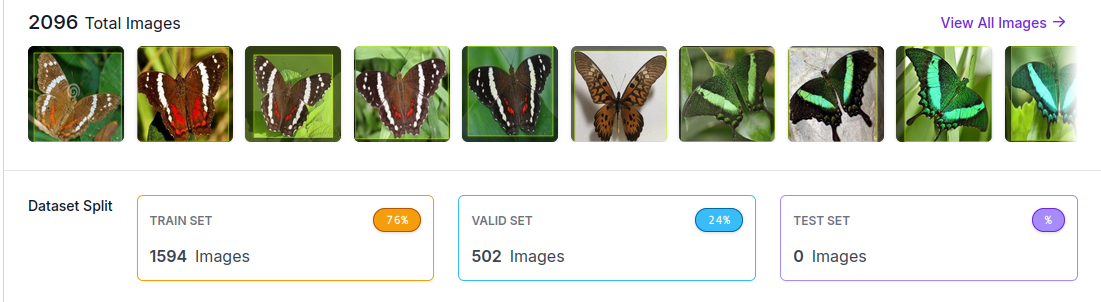
\includegraphics[width=0.8\textwidth]{trained_small_butterflies/dataset_simple}
    \end{center}
    The dataset only has a pre-process of resizing to 640.
    The relevant metrics for training and validation are shown in the figure~\ref{fig:results-small}.
    From the charts, specially from box\_loss and cls\_loss I can see that the model learns very rapidly from the train data and it also the learning is successful against the validation set.
    Since we are measuring only one class, precision and recall also are almost 1.0.
    The model looks perfect, but if I test it against the dataset from the Challenge, I've only got a poor accuracy of approximately 0.5.
    Using the inference of the model to infer from the images of the challenge and YouTube's video are in the figure~\ref{fig:trained_small_butterflies}
    It looks like the images from training and validation are quite similar, that is why it looks like there is an overfitting.
    \begin{figure}
        \begin{center}
            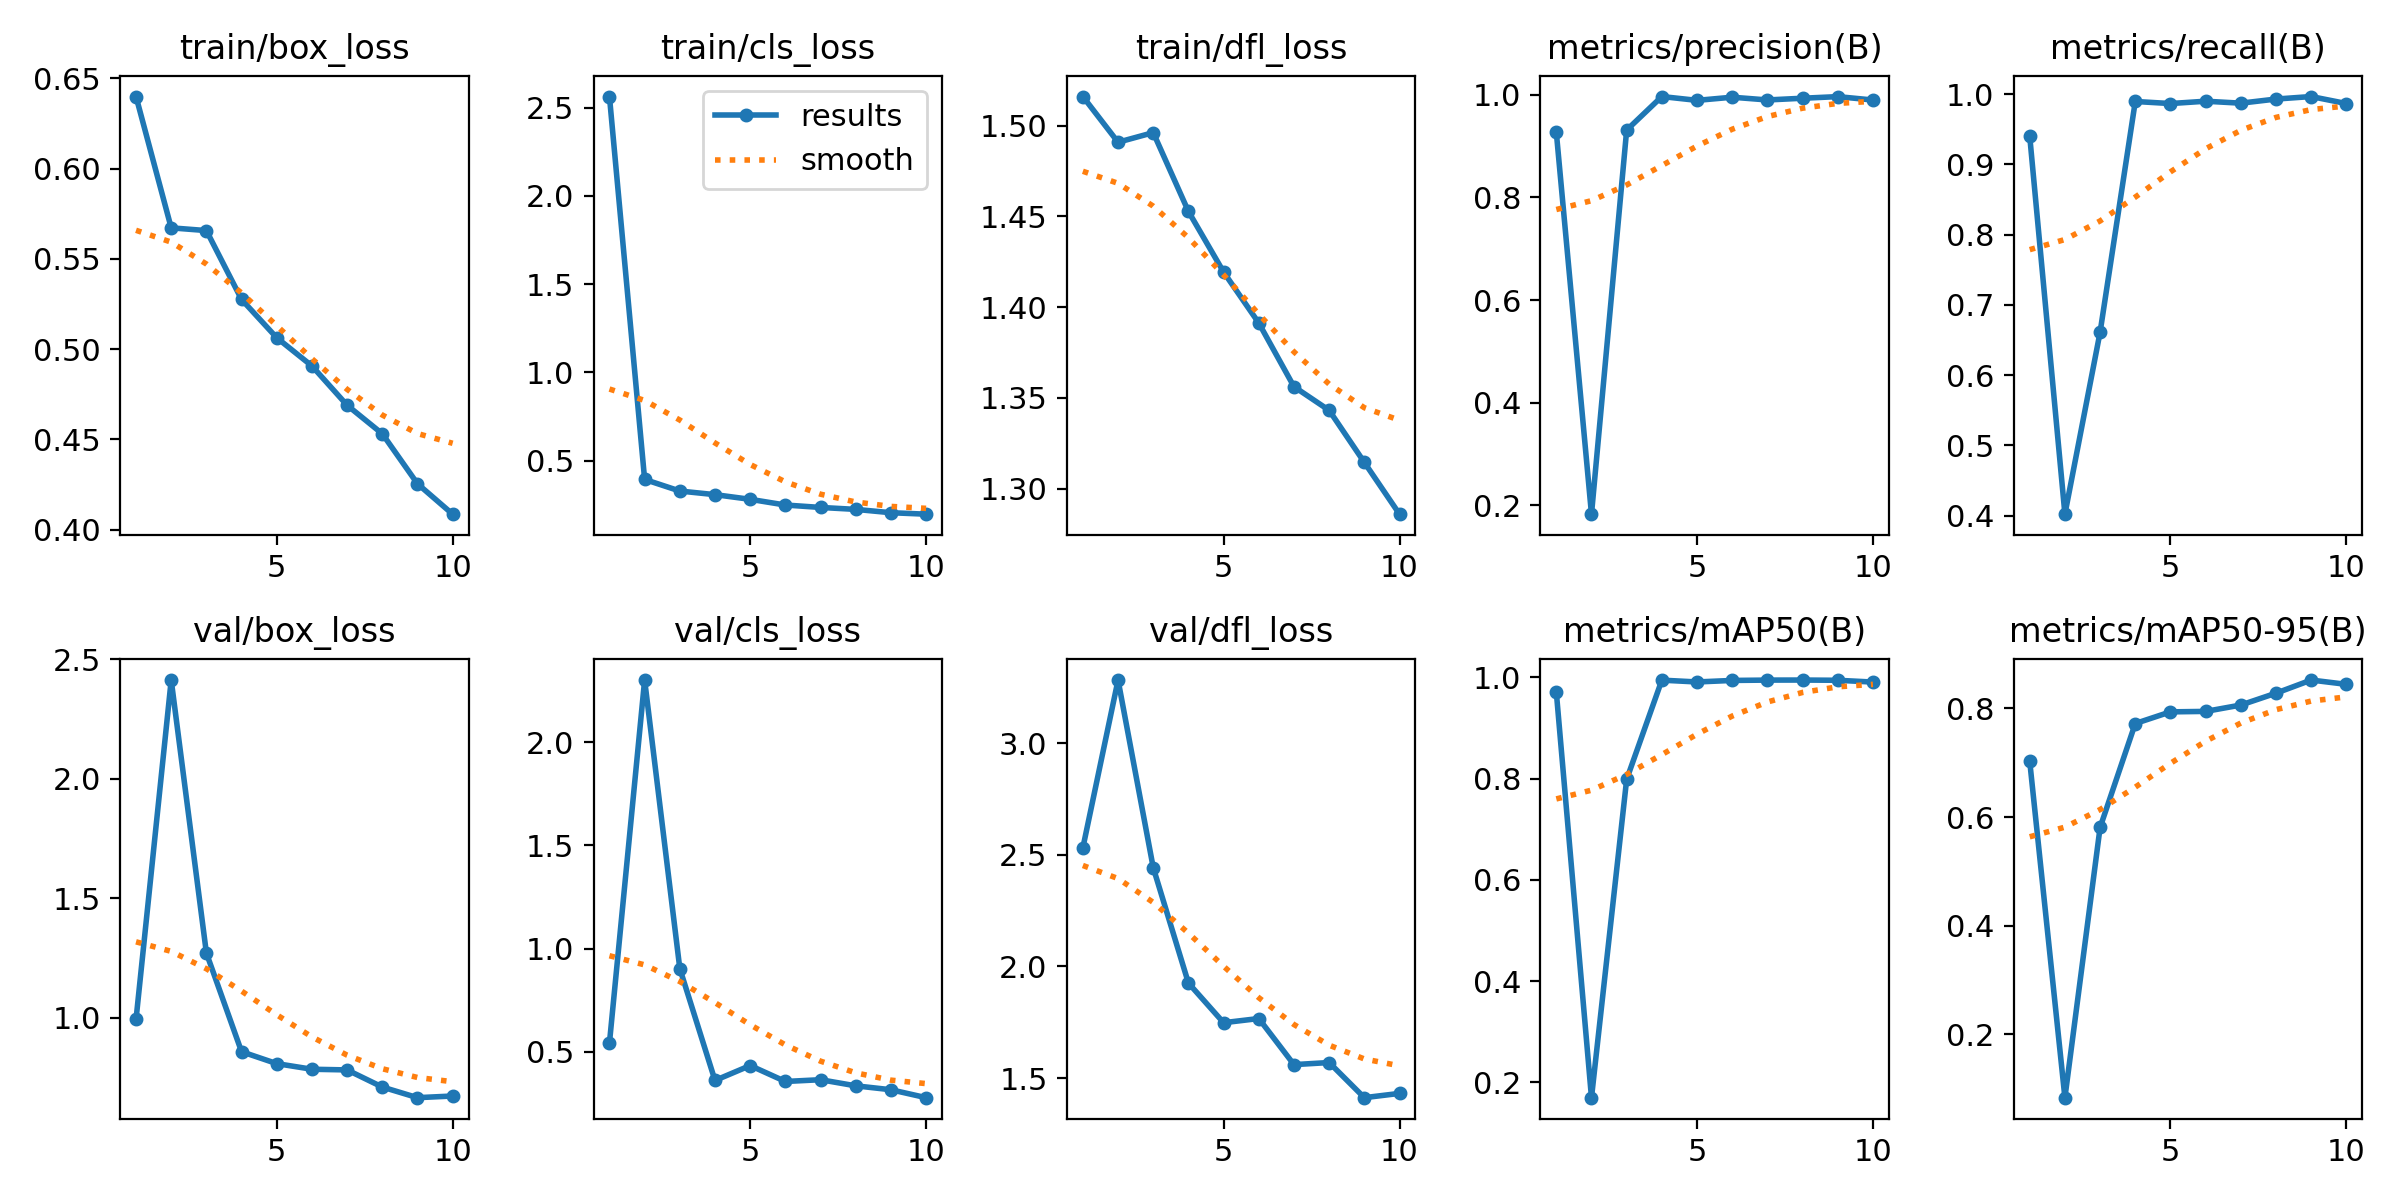
\includegraphics[width=0.8\textwidth]{trained_small_butterflies/results}
            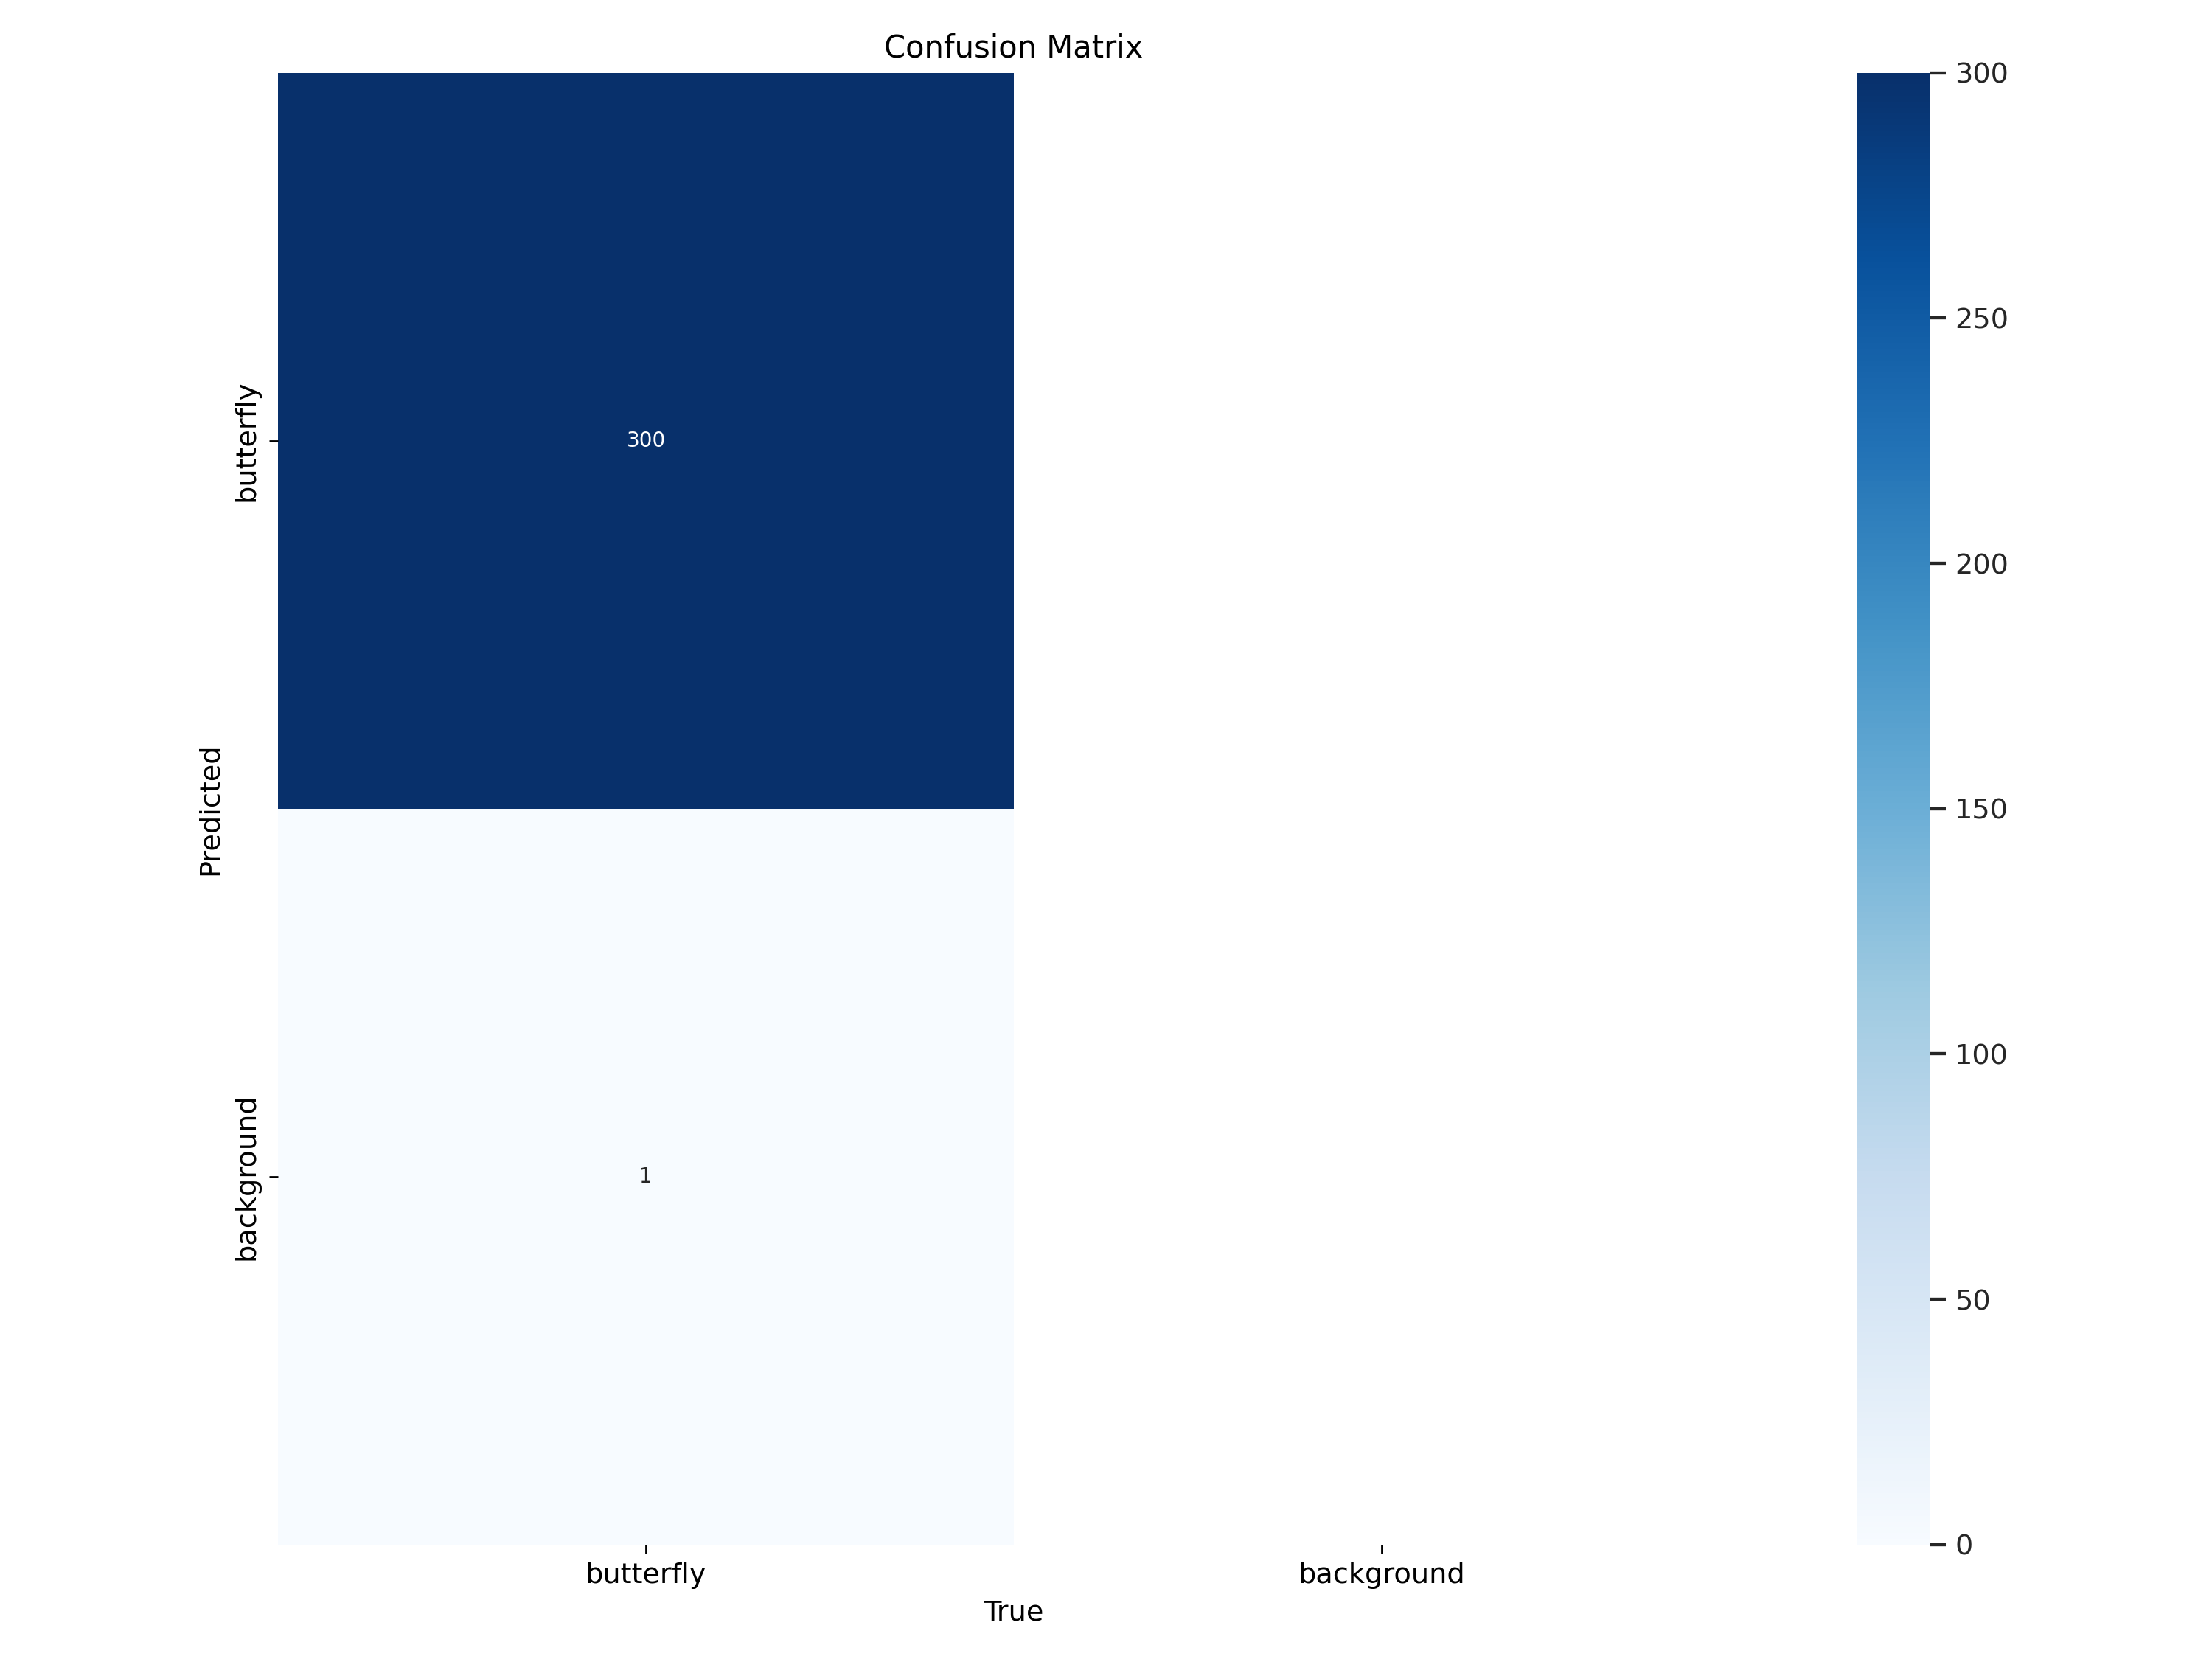
\includegraphics[width=0.4\textwidth]{trained_small_butterflies/confusion_matrix_simple}
        \end{center}
        \caption{Result of training of the small dataset of butterflies.}
        \label{fig:results-small}
    \end{figure}
    \begin{figure}
        \begin{subfigure}{.9\textwidth}
            \centering
            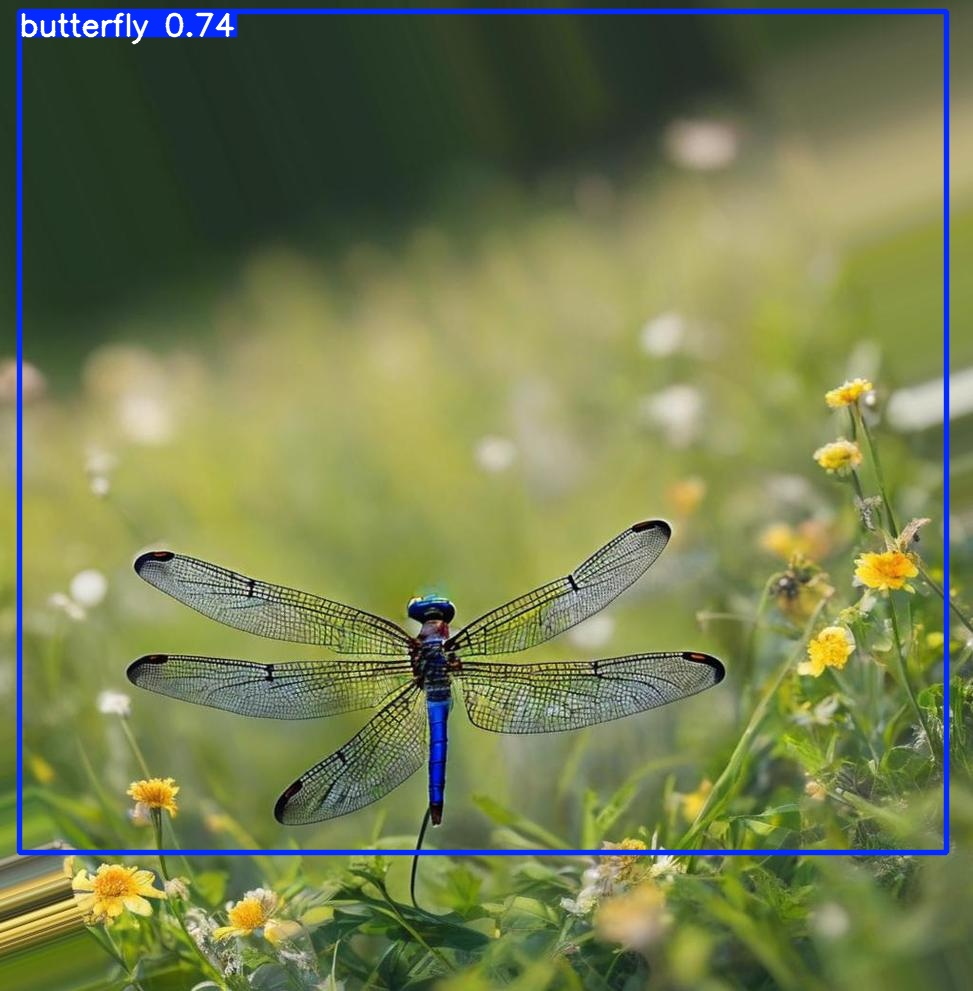
\includegraphics[width=.4\linewidth]{trained_small_butterflies/negative_imagen_723}
            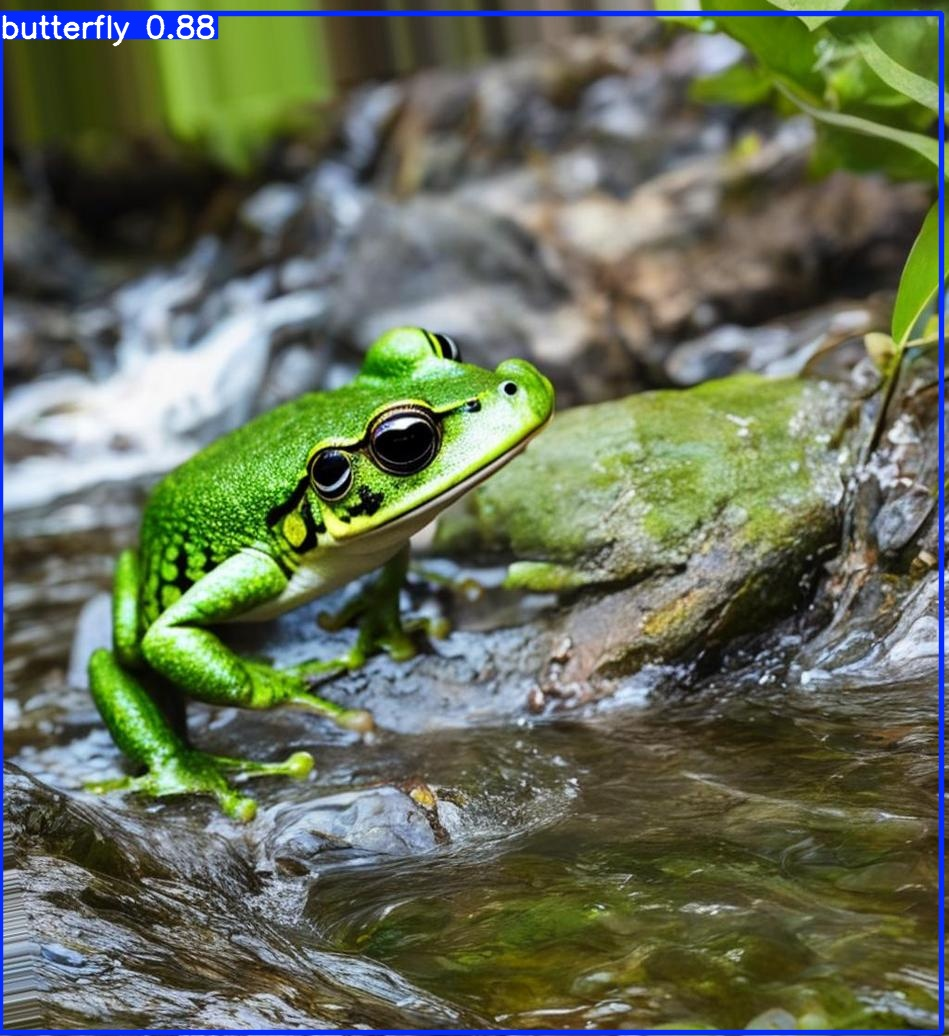
\includegraphics[width=.4\linewidth]{trained_small_butterflies/negative_imagen_880}
            \caption{Negative class in the training data of the challenge}
            \label{fig:negative-trained_small_butterflies}
        \end{subfigure}

        \begin{subfigure}{.9\textwidth}
            \centering
            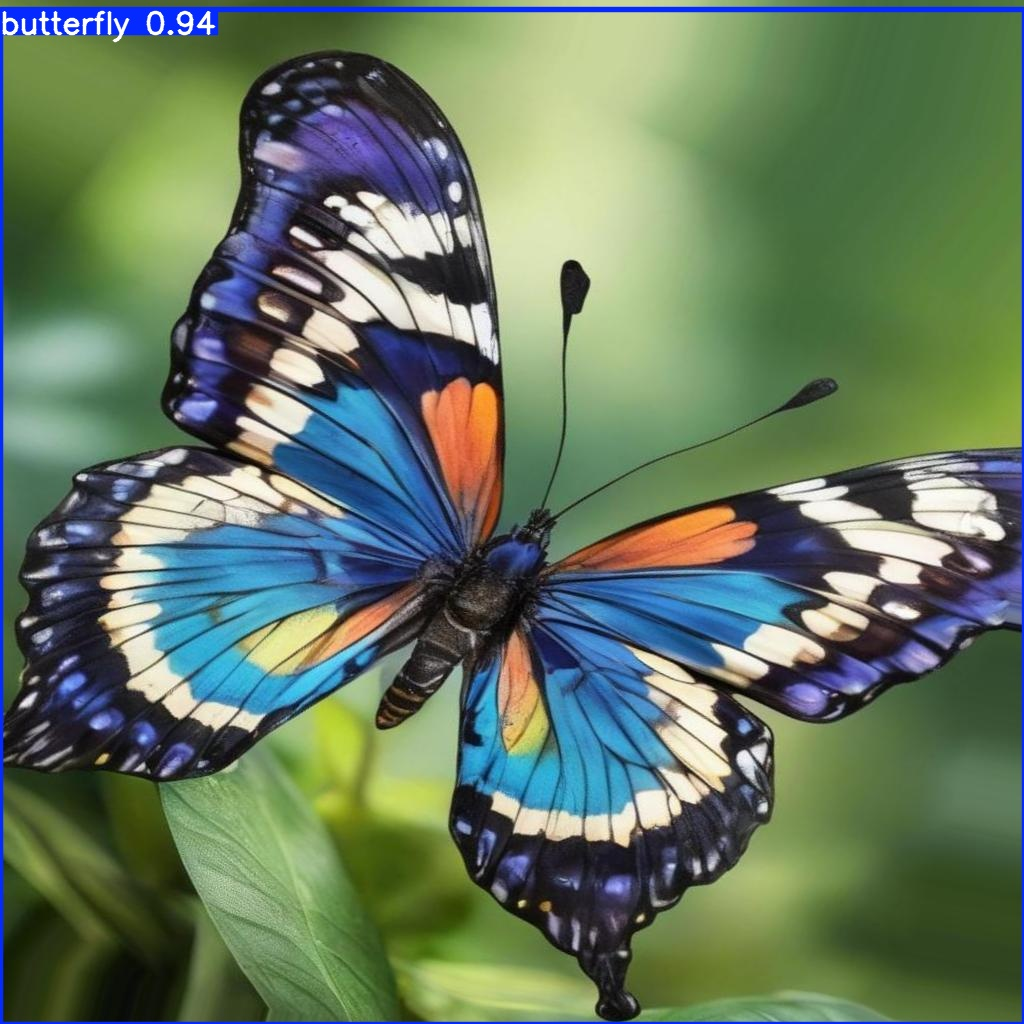
\includegraphics[width=.4\linewidth]{trained_small_butterflies/positive_imagen_45}
            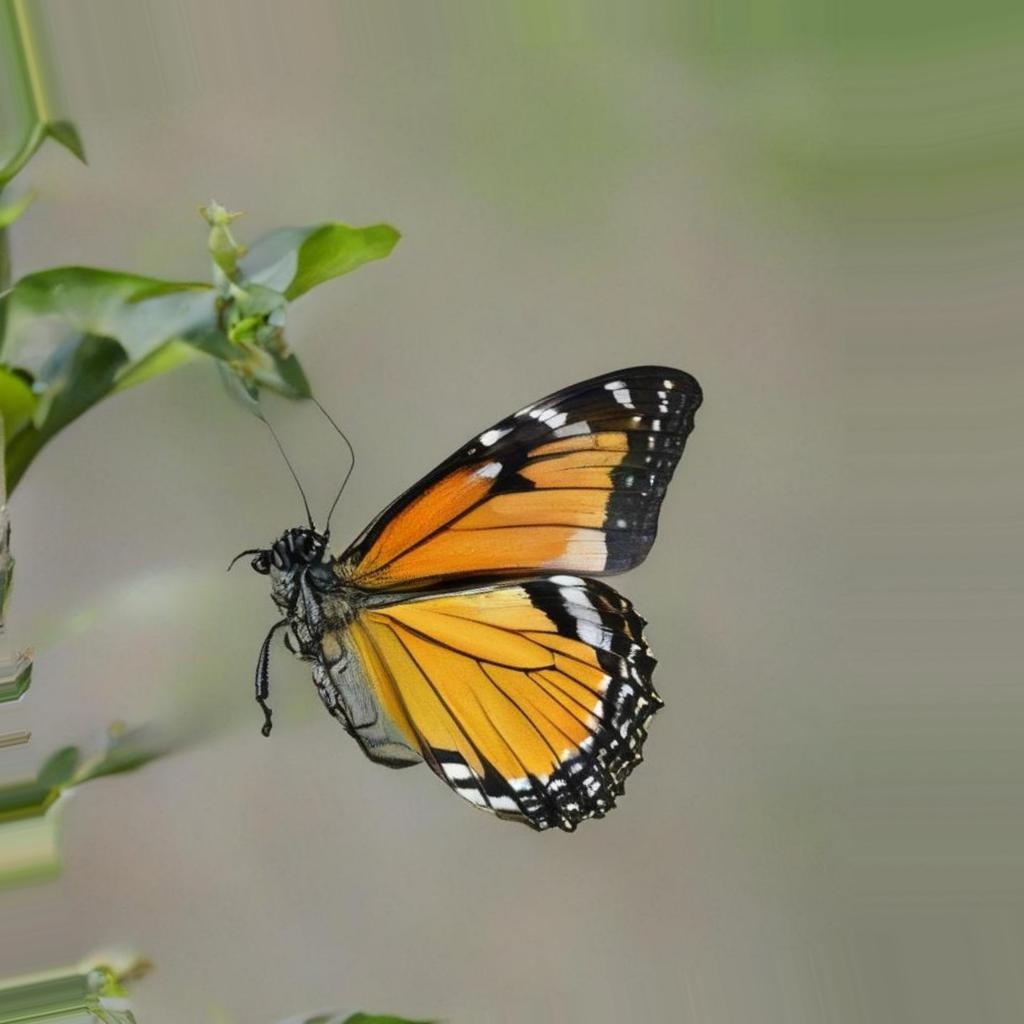
\includegraphics[width=.4\linewidth]{trained_small_butterflies/positive_imagen_888}
            \caption{Positive class in the training data of the challenge}
            \label{fig:positive-trained_small_butterflies}
        \end{subfigure}

        \begin{subfigure}{.9\textwidth}
            \centering
            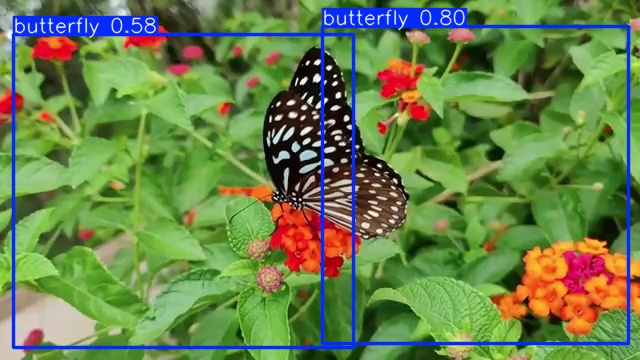
\includegraphics[width=.4\linewidth]{trained_small_butterflies/photogram_16}
            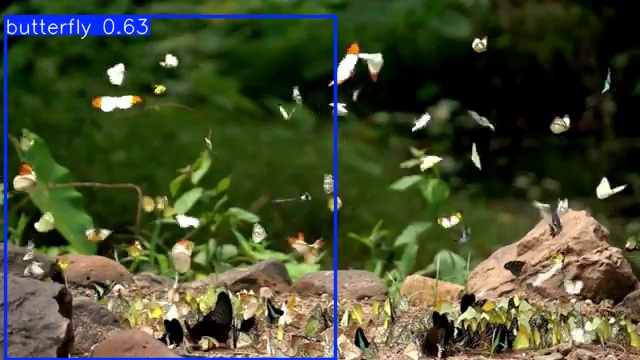
\includegraphics[width=.4\linewidth]{trained_small_butterflies/photogram_93}
            \caption{Images of the YouTube video}
            \label{fig:video-trained_small_butterflies}
        \end{subfigure}
        \caption{Images results using transfer learning using the small dataset of butterflies}
        \label{fig:trained_small_butterflies}
    \end{figure}

    \newpage
    Continuing the same problem but with extra-dataset, I've found an extra-dataset and I managed to merge using RoboFlow.
    \begin{center}
        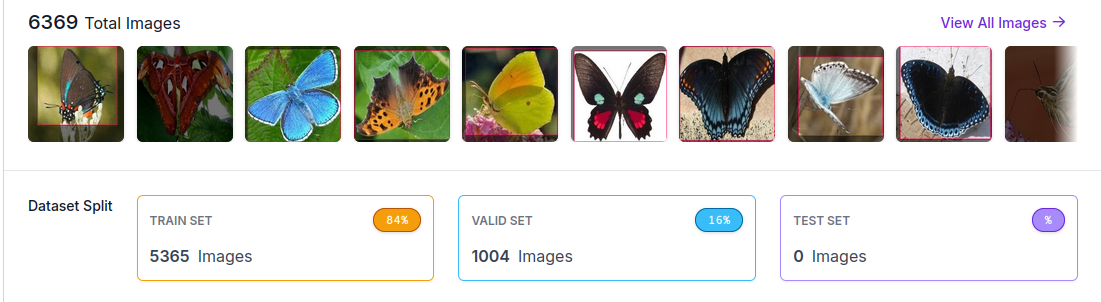
\includegraphics[width=0.8\textwidth]{trained_bigger_butterflies/dataset_enhanced}
    \end{center}
    The dataset only has a pre-process of resizing to 640.
    The relevant metrics for training and validation are shown in the figure~\ref{fig:results-big}.
    From the charts, specially from box\_loss and cls\_loss I can see that the during the training it learns fast but the validation do not follow.
    Specially val/cls\_loss, it got stuck.
    Since we are measuring only one class, precision is over 0.8 and recall also are almost 1.0.
    The model, again,  looks perfect, but if I test it against the dataset from the Challenge, I've only got a poor accuracy of approximately 0.52.
    Which is an improvement from the previous model.
    Using the inference of the model to infer from the images of the challenge and YouTube's video are in the figure~\ref{fig:trained_bigger_butterflies}
    Again, it looks like the images from training and validation are quite similar, that is why it looks like there is an overfitting.
    \begin{figure}
        \begin{center}
            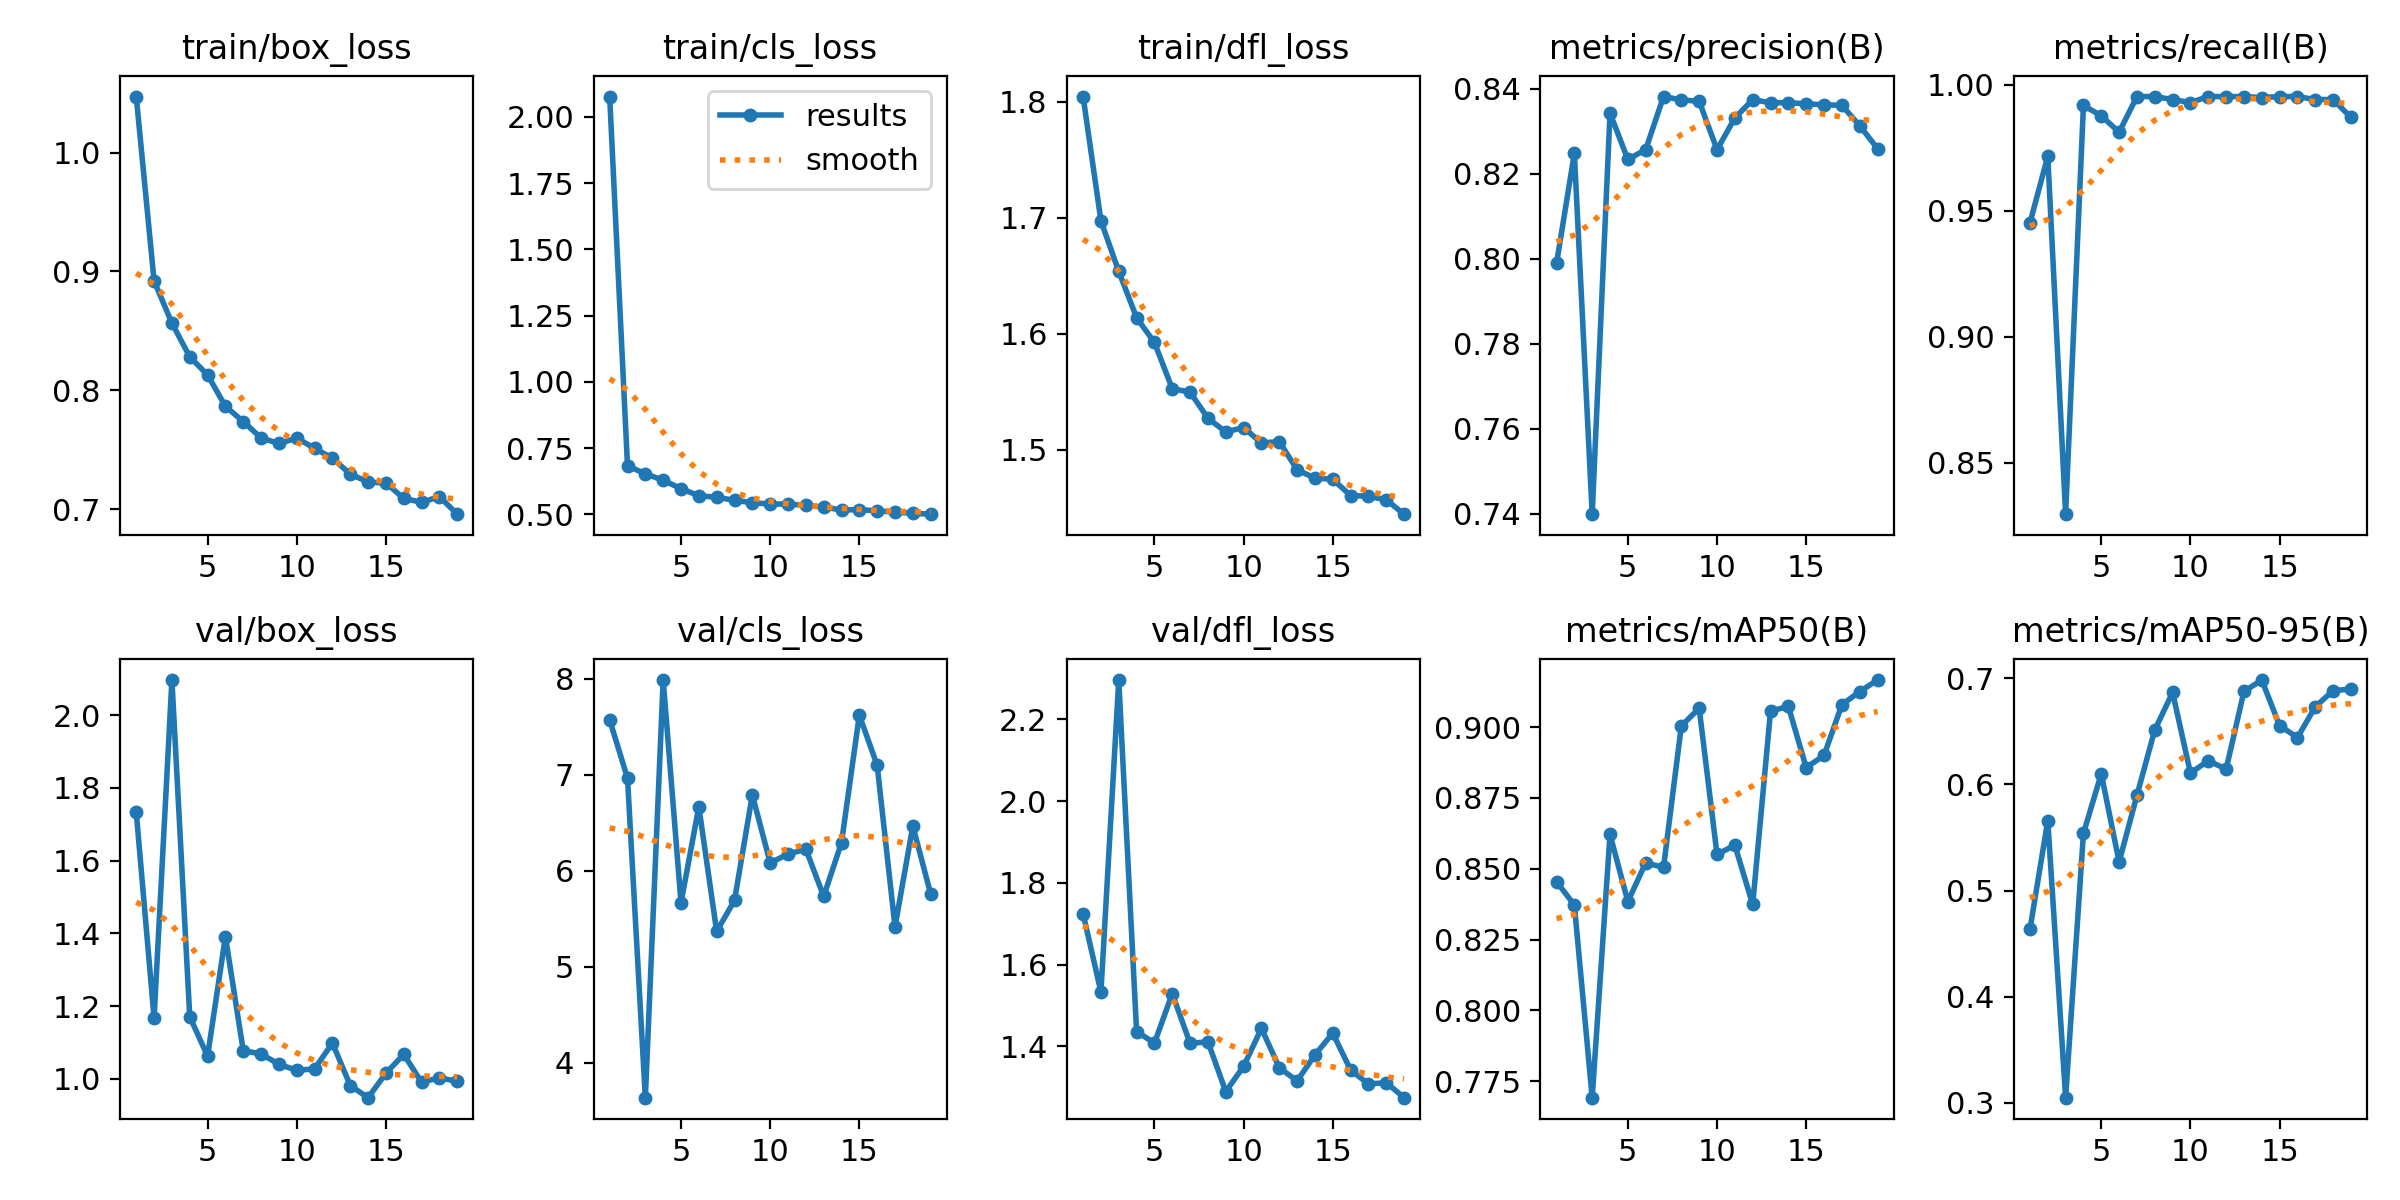
\includegraphics[width=0.8\textwidth]{trained_bigger_butterflies/results}
            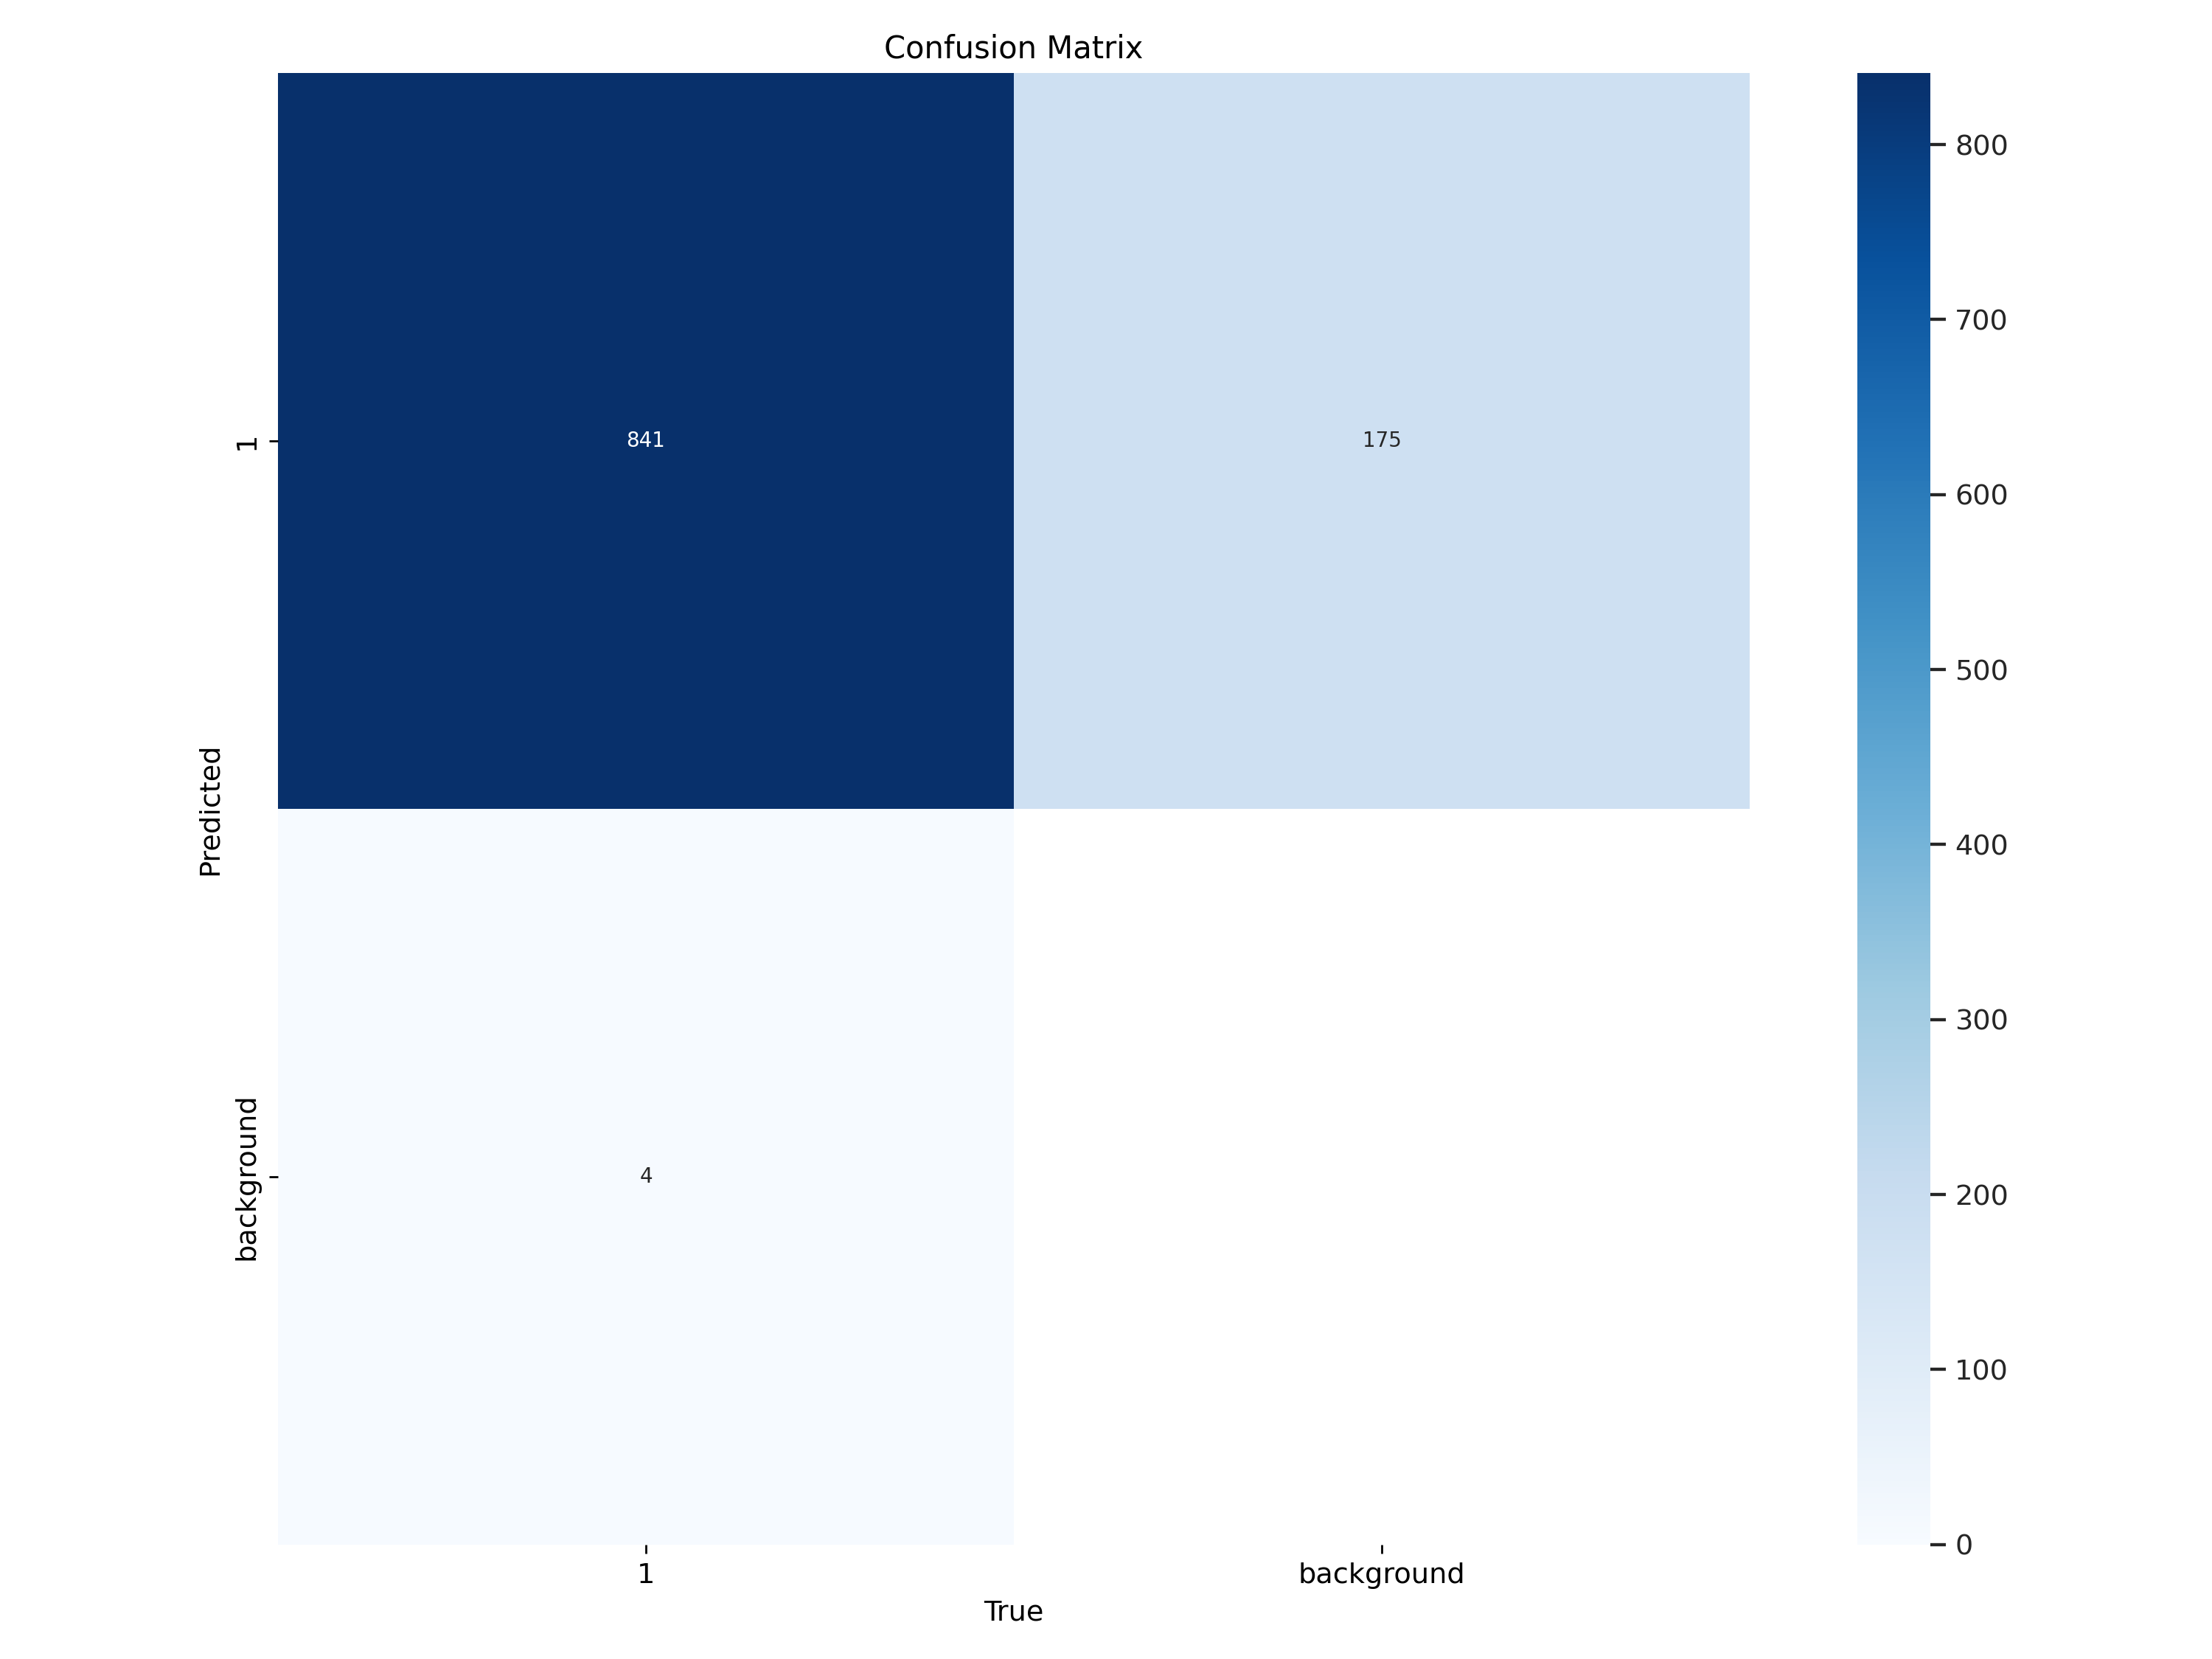
\includegraphics[width=0.4\textwidth]{trained_bigger_butterflies/confusion_matrix}
        \end{center}
        \caption{Result of training of the small dataset of butterflies.}
        \label{fig:results-big}
    \end{figure}
    \begin{figure}
        \begin{subfigure}{.9\textwidth}
            \centering
            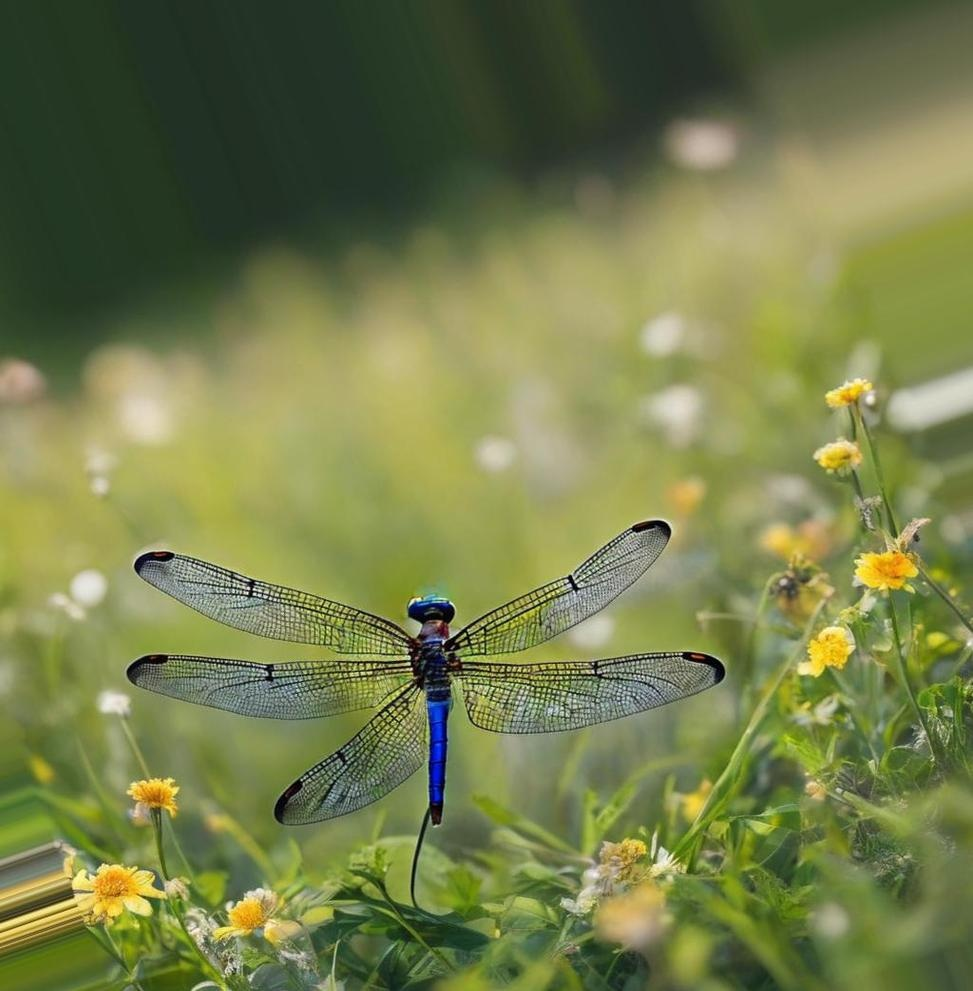
\includegraphics[width=.4\linewidth]{trained_bigger_butterflies/negative_imagen_723}
            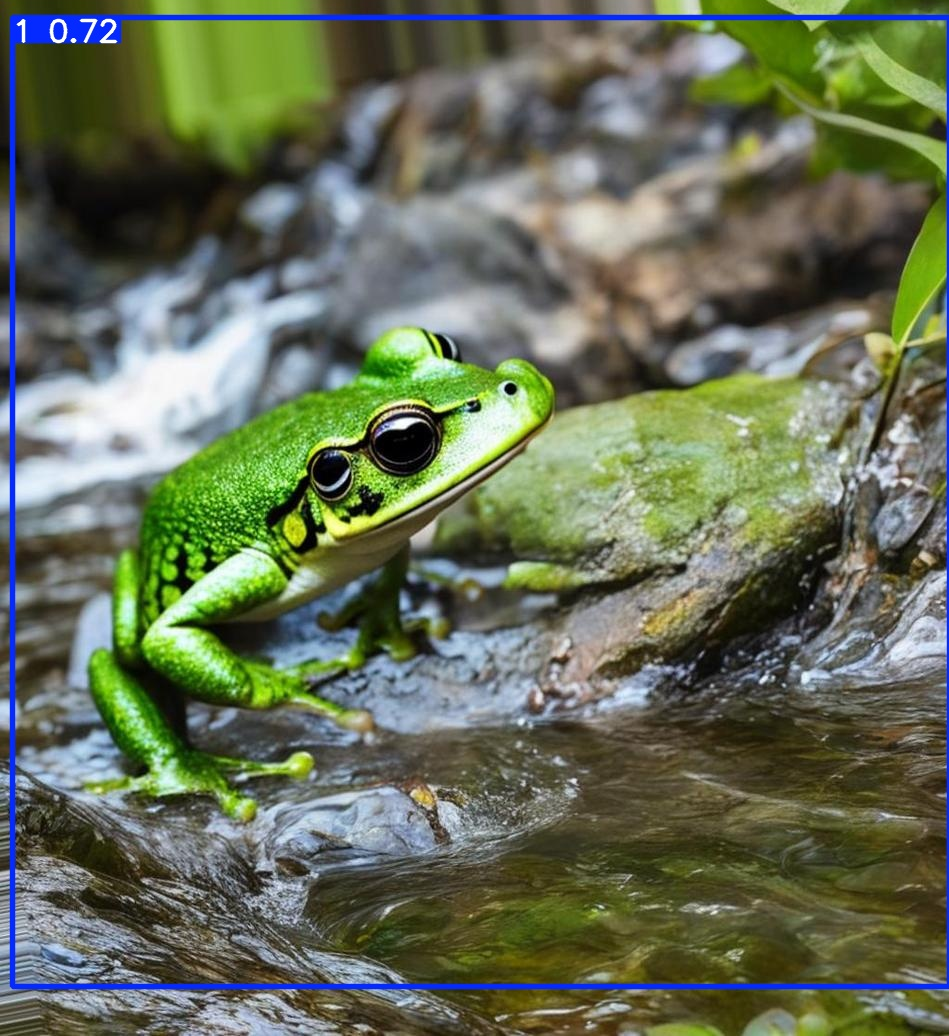
\includegraphics[width=.4\linewidth]{trained_bigger_butterflies/negative_imagen_880}
            \caption{Negative class in the training data of the challenge}
            \label{fig:negative-trained_bigger_butterflies}
        \end{subfigure}

        \begin{subfigure}{.9\textwidth}
            \centering
            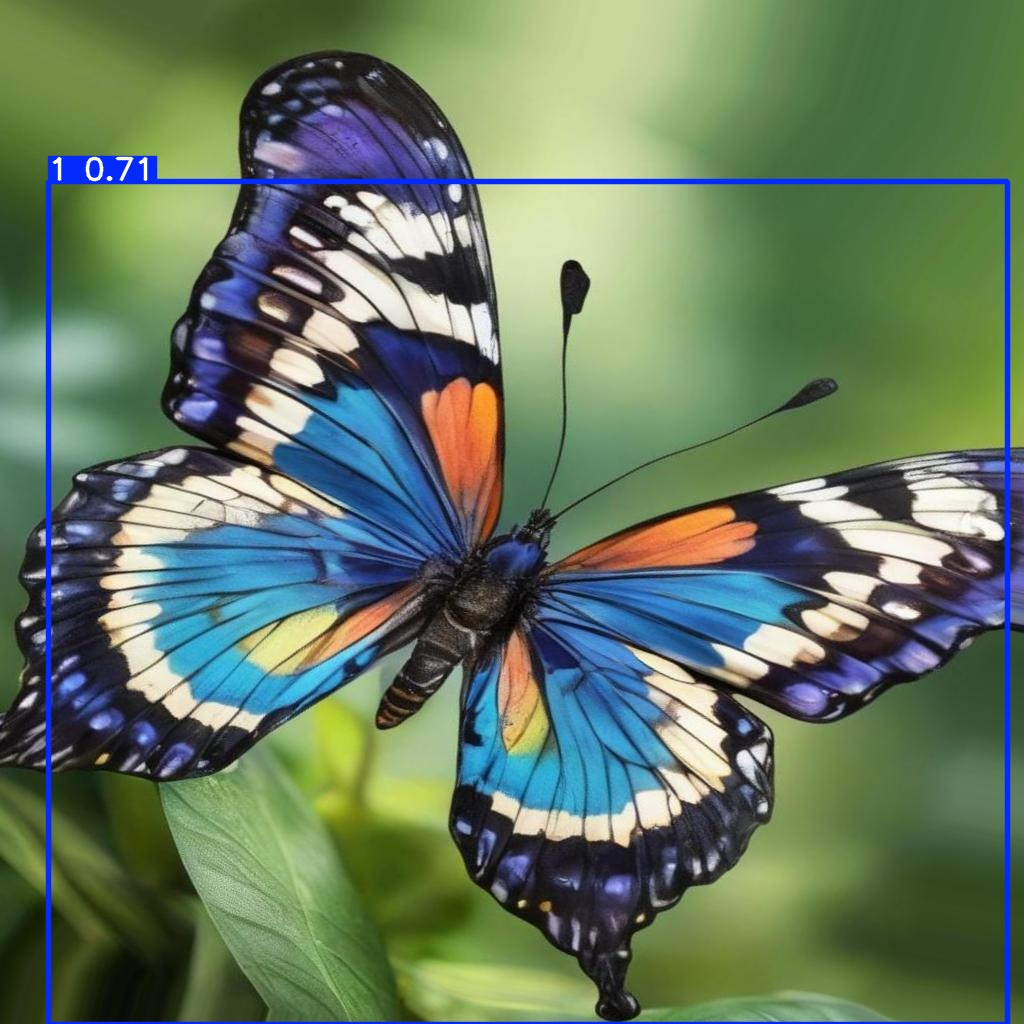
\includegraphics[width=.4\linewidth]{trained_bigger_butterflies/positive_imagen_45}
            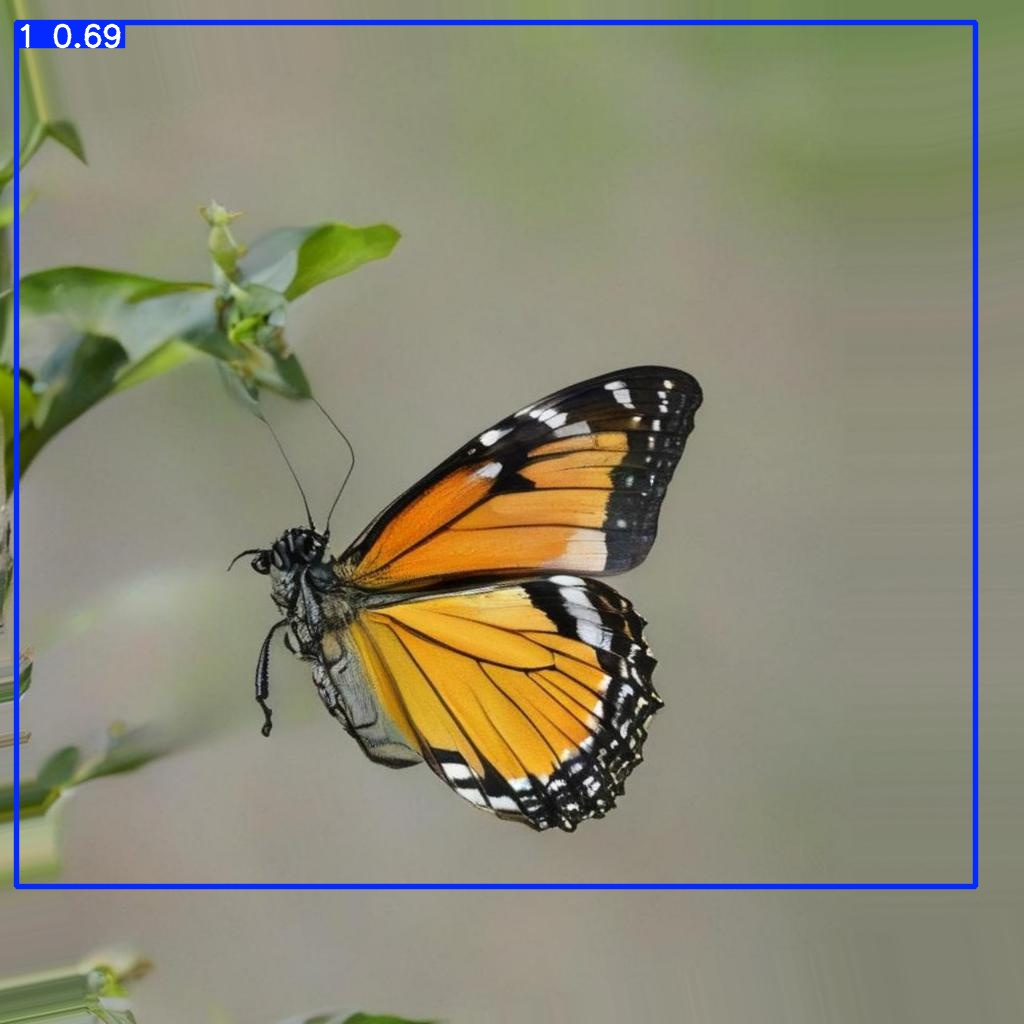
\includegraphics[width=.4\linewidth]{trained_bigger_butterflies/positive_imagen_888}
            \caption{Positive class in the training data of the challenge}
            \label{fig:positive-trained_bigger_butterflies}
        \end{subfigure}

        \begin{subfigure}{.9\textwidth}
            \centering
            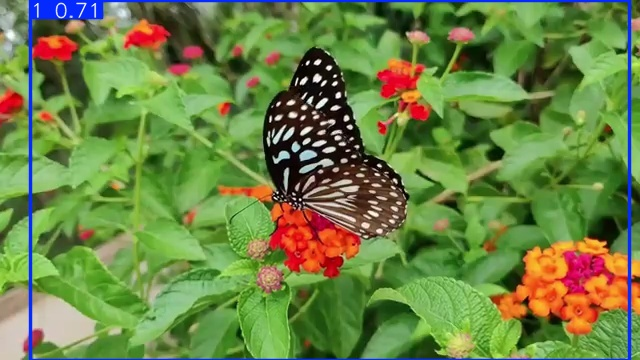
\includegraphics[width=.4\linewidth]{trained_bigger_butterflies/photogram_16}
            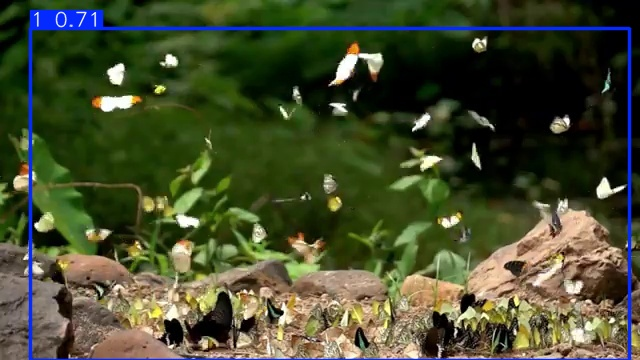
\includegraphics[width=.4\linewidth]{trained_bigger_butterflies/photogram_93}
            \caption{Images of the YouTube video}
            \label{fig:video-trained_bigger_butterflies}
        \end{subfigure}
        \caption{Images results using transfer learning using the doble/big dataset of butterflies}
        \label{fig:trained_bigger_butterflies}
    \end{figure}

    \newpage
    \textbf{Transfer learning to detect two novel classes}
    For this experiment, I used the dataset of butterflies and moths.
    \begin{center}
        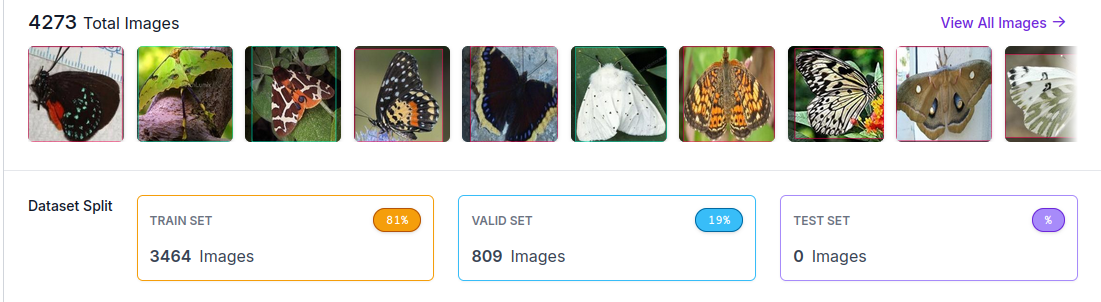
\includegraphics[width=0.8\textwidth]{trained_two_classes/dataset_two_classes}
    \end{center}
    The dataset only has a pre-process of resizing to 640.
    But during the training, it was resized to 1024 by the library of Yolo.
    The relevant metrics for training and validation are shown in the figure~\ref{fig:results-two-classes}.
    From the charts, it looks like the hyper-parameters are correct, because the validation metrics follow to the acquired by training.
    Since in this case I am measuring two classes and I care more precision, the analysis of the precision curve is relevant.
    In the figure~\ref{fig:results-two-classes} I can extract that a confidence of 60\% or 0.6 is enough to capture many of the characteristics.
    I can also get to that conclusions from the mAP50 y mAP50-95 charts.
    In this case the model do not look perfect, but is fine for the validation set.
    Talking about the challenge of classification of butterflies.
    What if I assume a detection of a month is equivalent to the detection of a butterfly.
    I test this hypothesis against the dataset from the Challenge, I've only got a poor accuracy of approximately 0.52.
    Which is the same value from the previous experiment.
    Reviewing the data from the Challenge, the images look like very synthetic.
    Maybe this is the reason why the low metrics.
    Using the inference of the model to infer from the images of the challenge and YouTube's video are in the figure~\ref{fig:trained_two_classes}
    \begin{figure}
        \begin{center}
            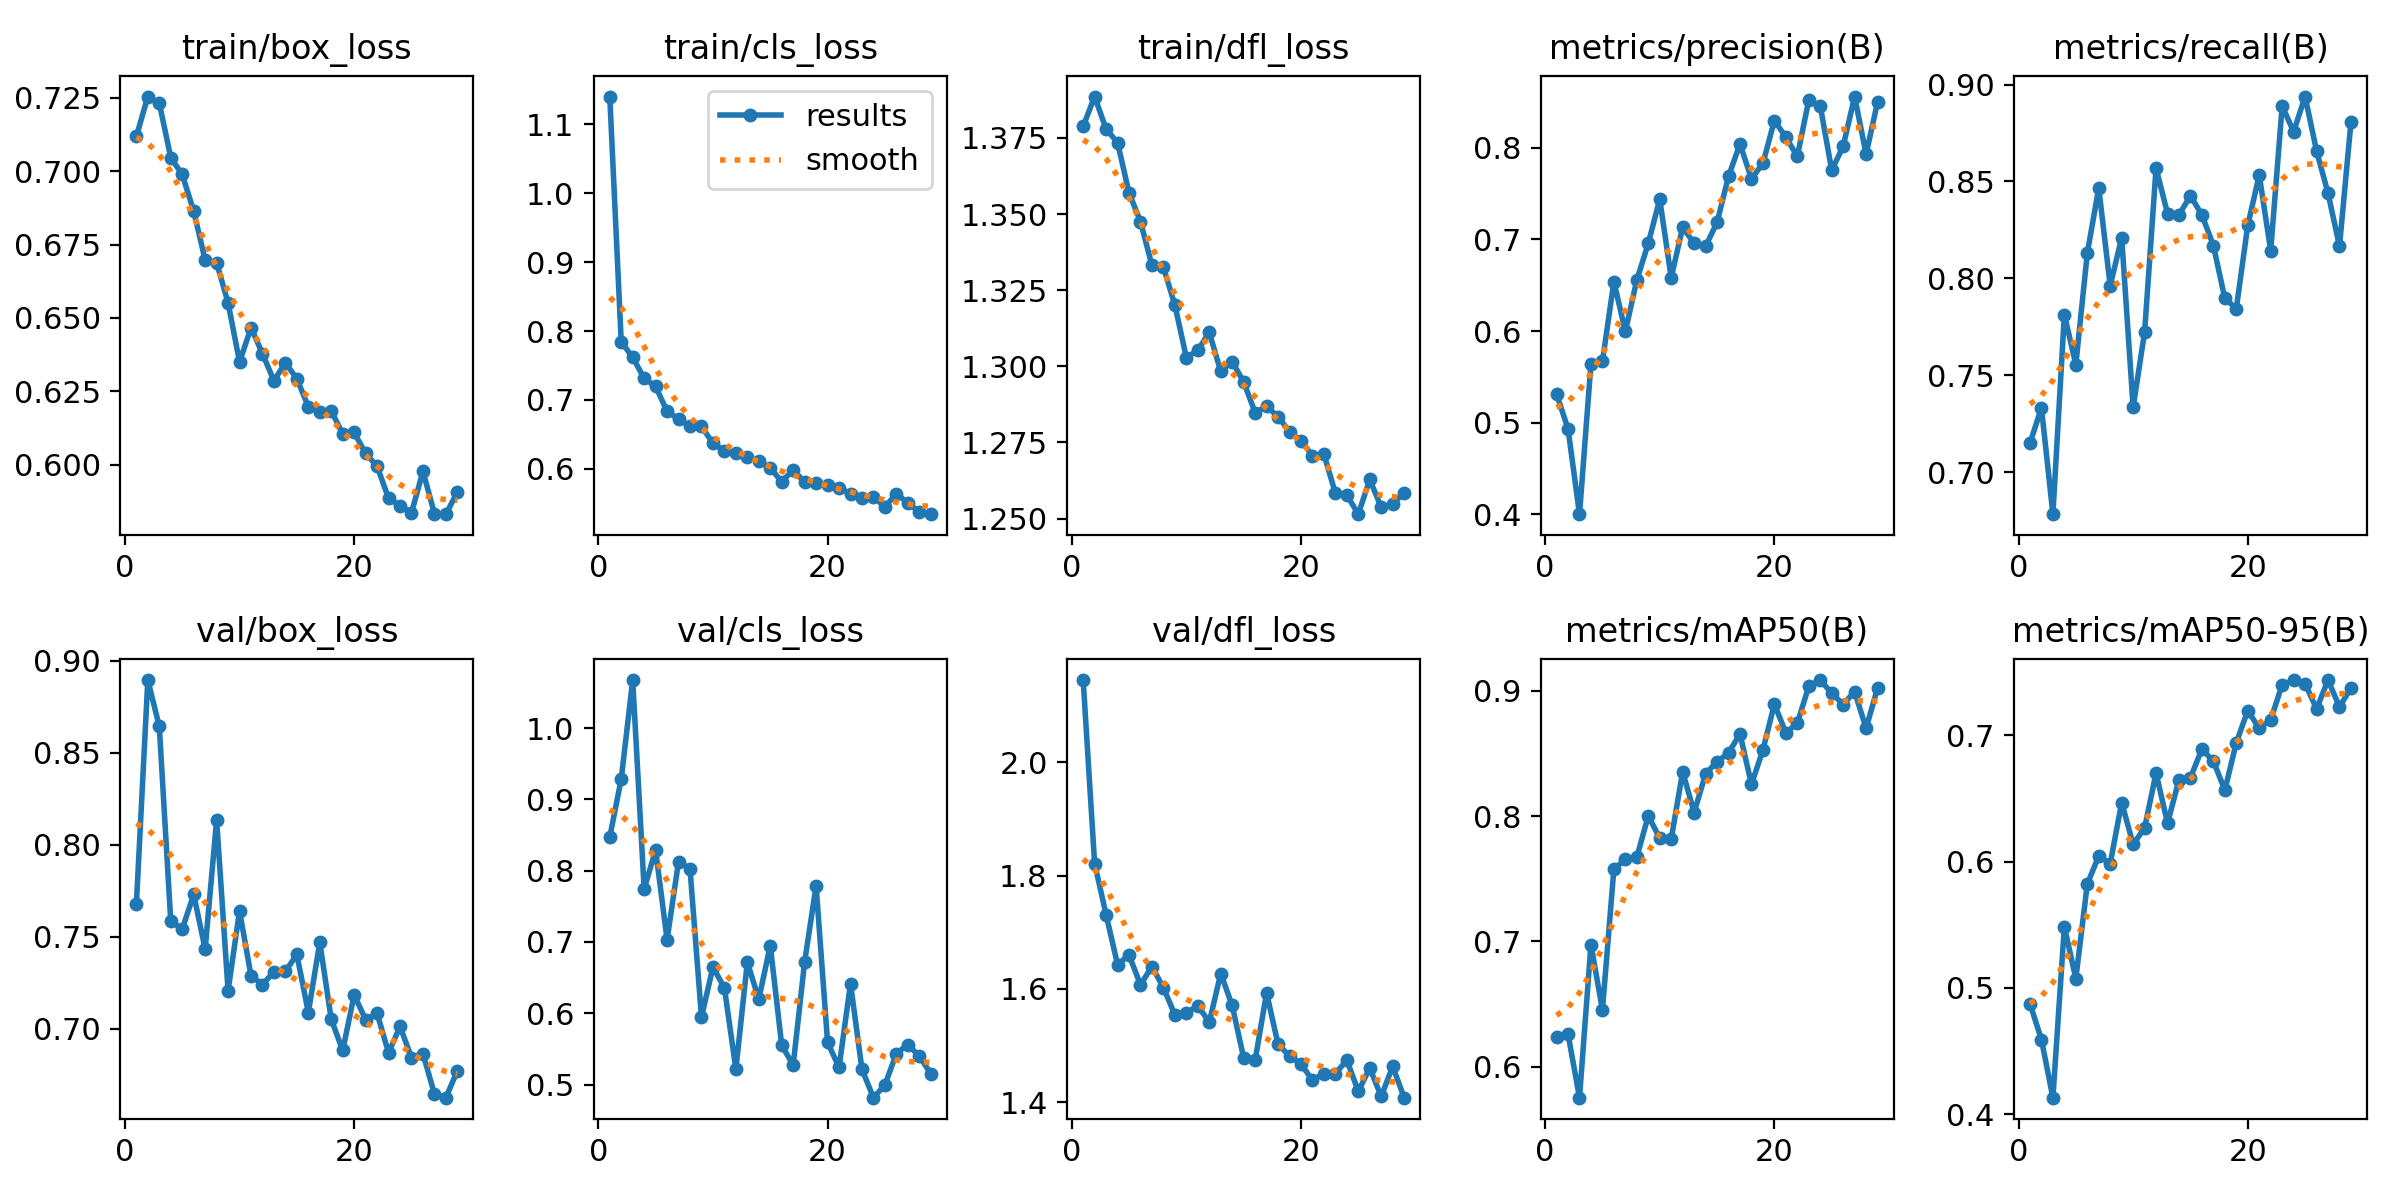
\includegraphics[width=0.8\textwidth]{trained_two_classes/results}
            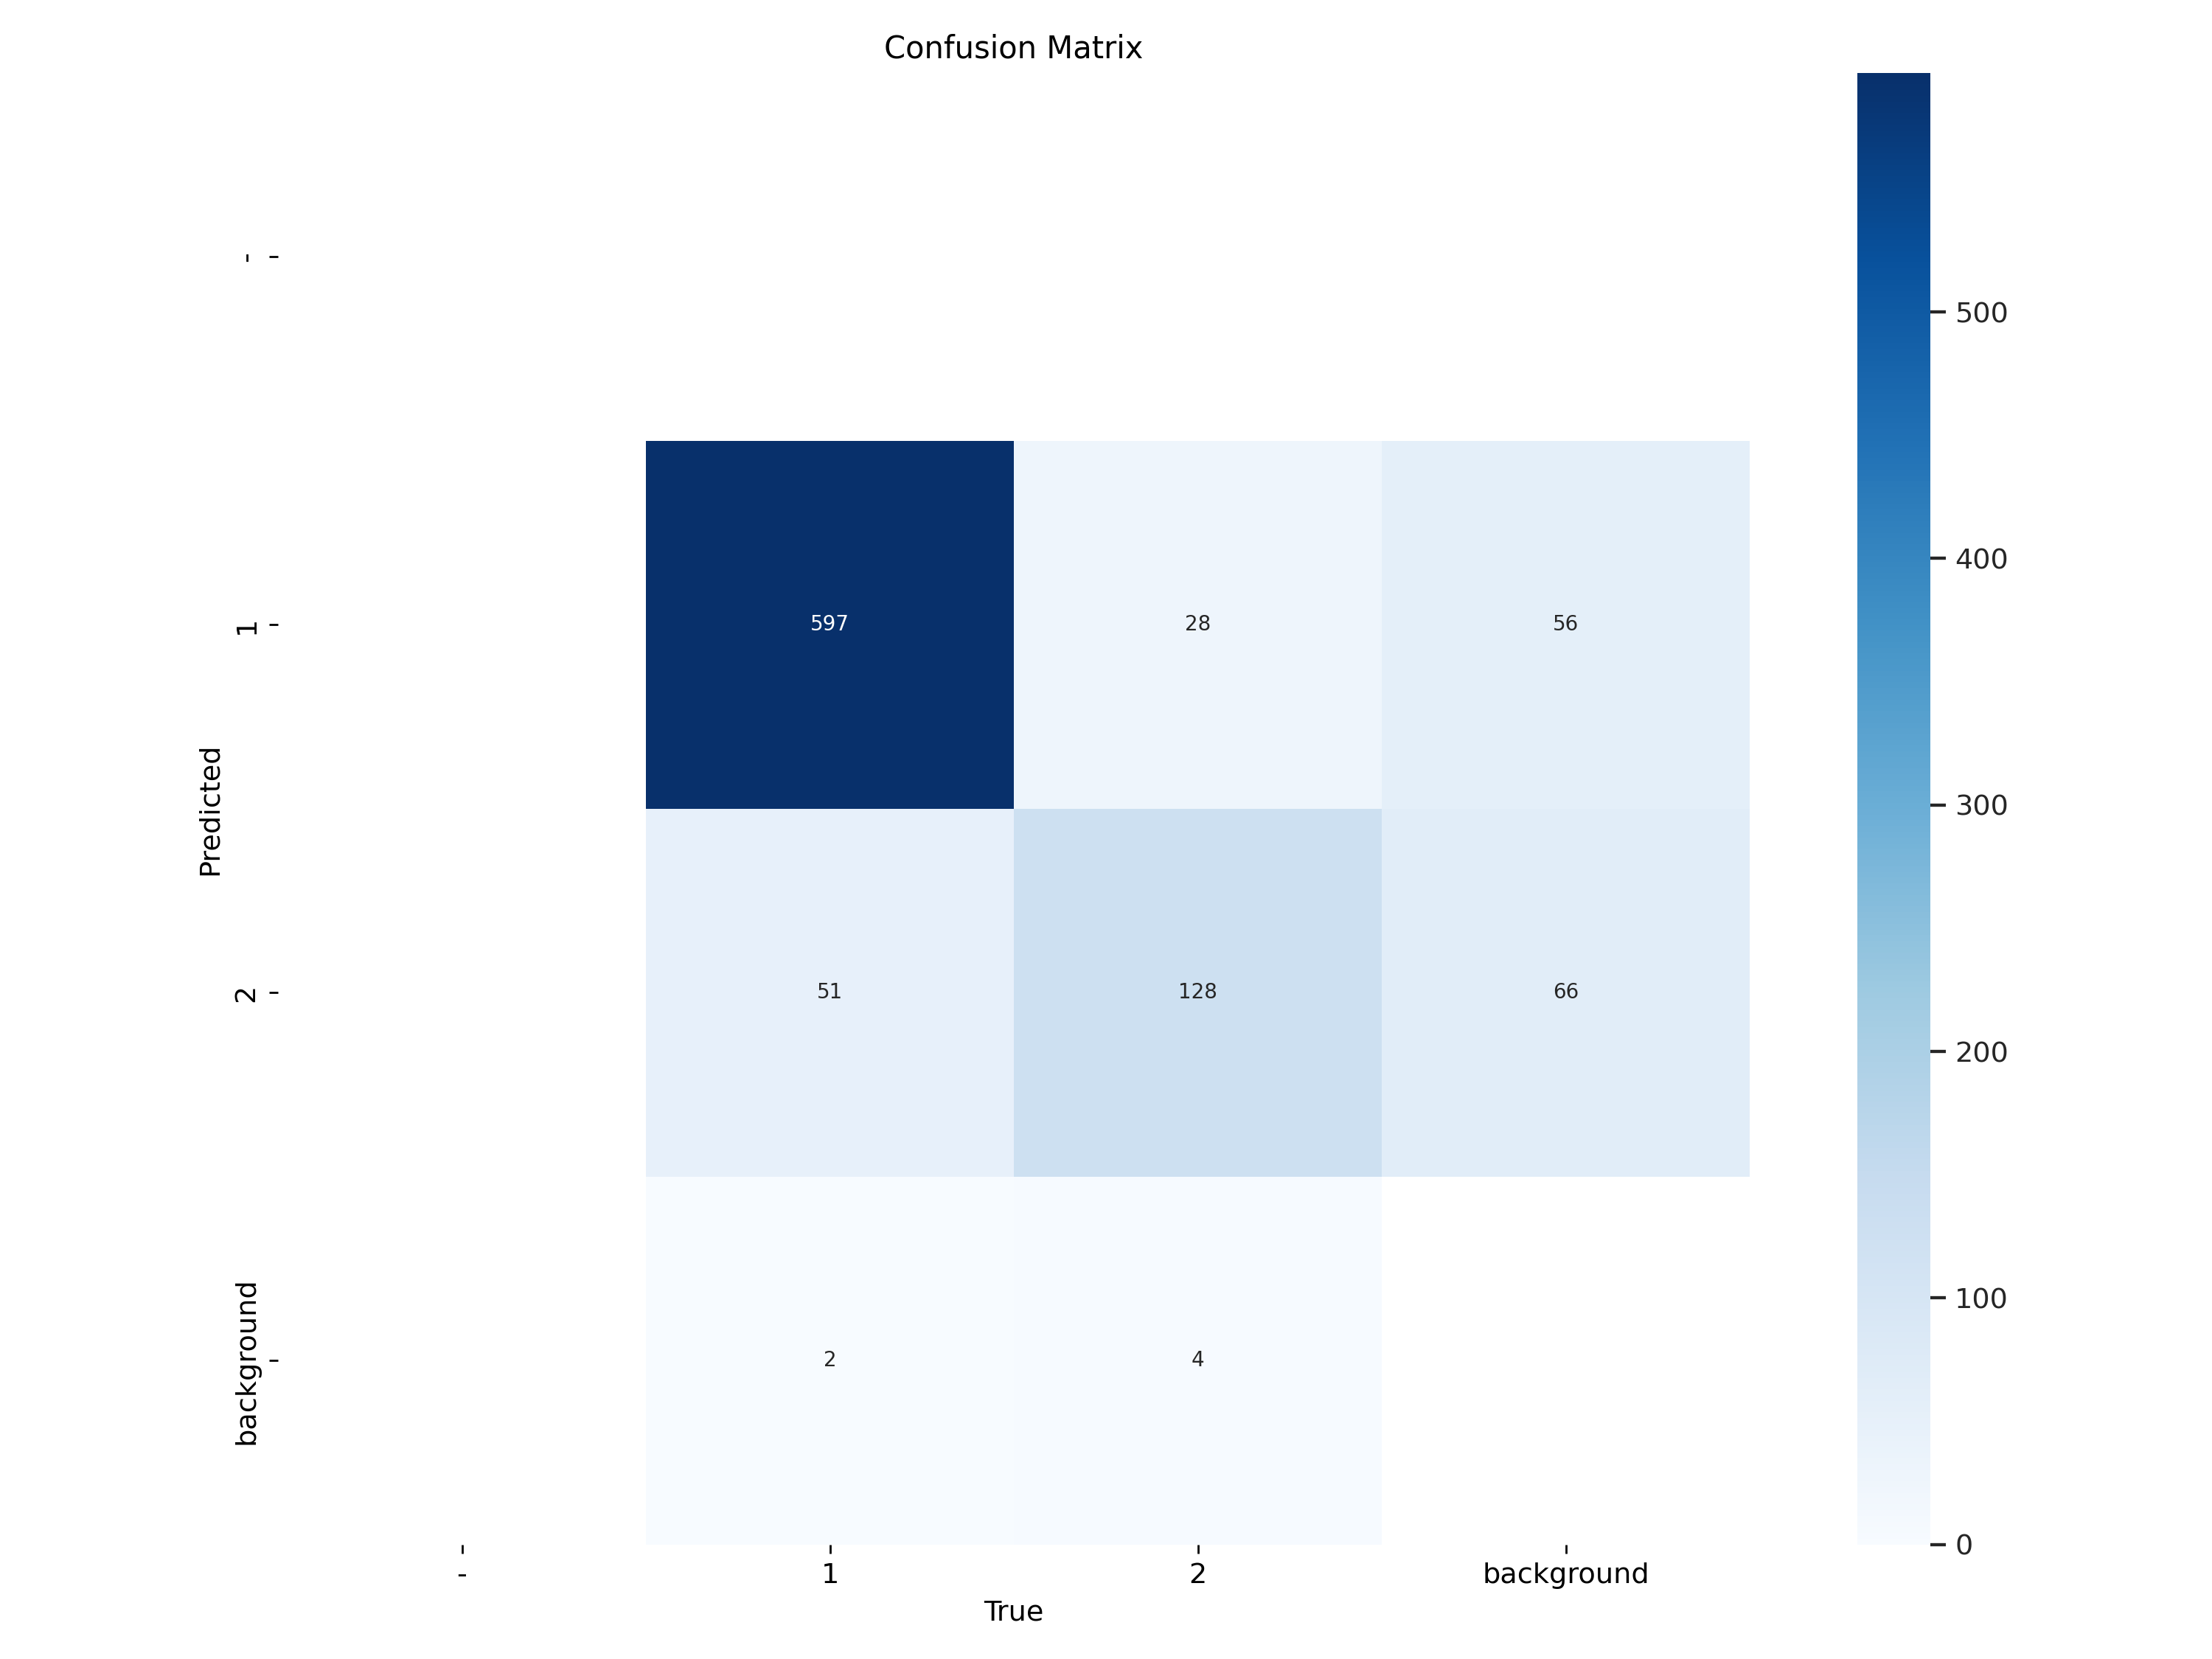
\includegraphics[width=0.4\textwidth]{trained_two_classes/confusion_matrix}
        \end{center}
        \caption{Result of training of the small dataset of butterflies.}
        \label{fig:results-two-classes}
    \end{figure}
    \begin{figure}
        \begin{subfigure}{.9\textwidth}
            \centering
            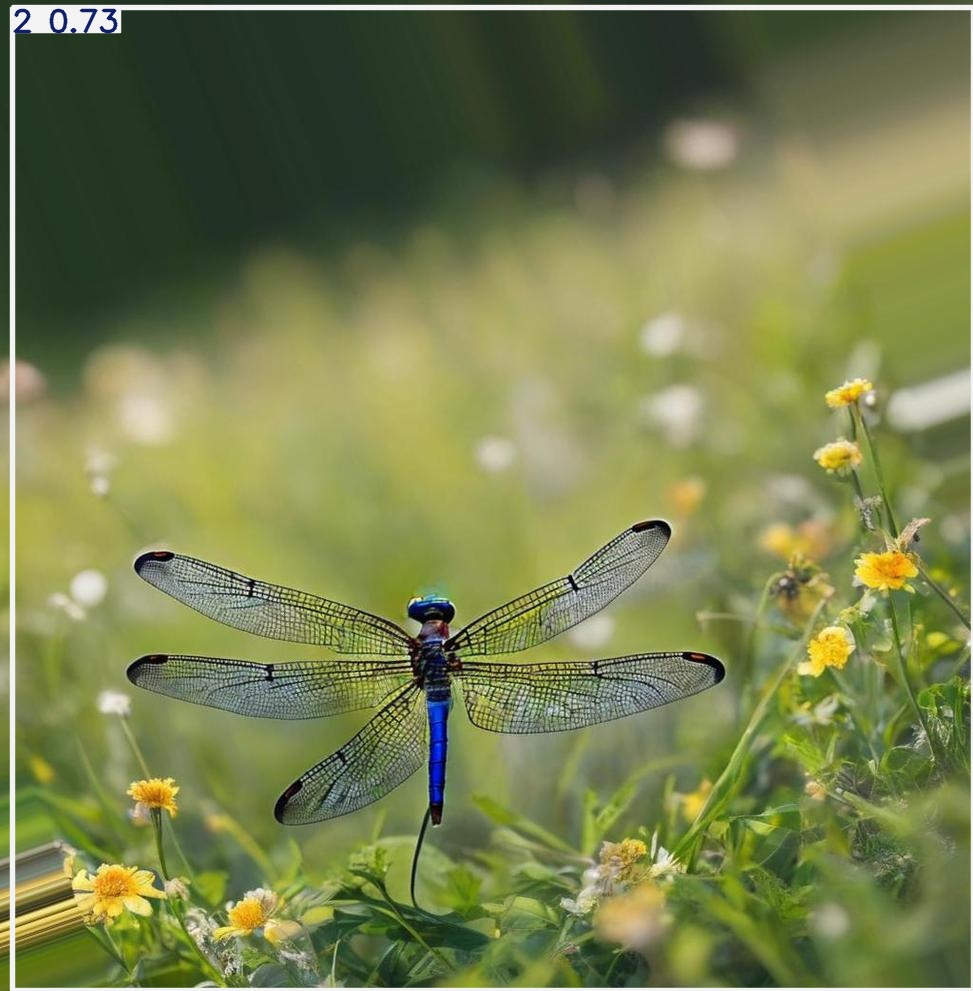
\includegraphics[width=.4\linewidth]{trained_two_classes/negative_imagen_723}
            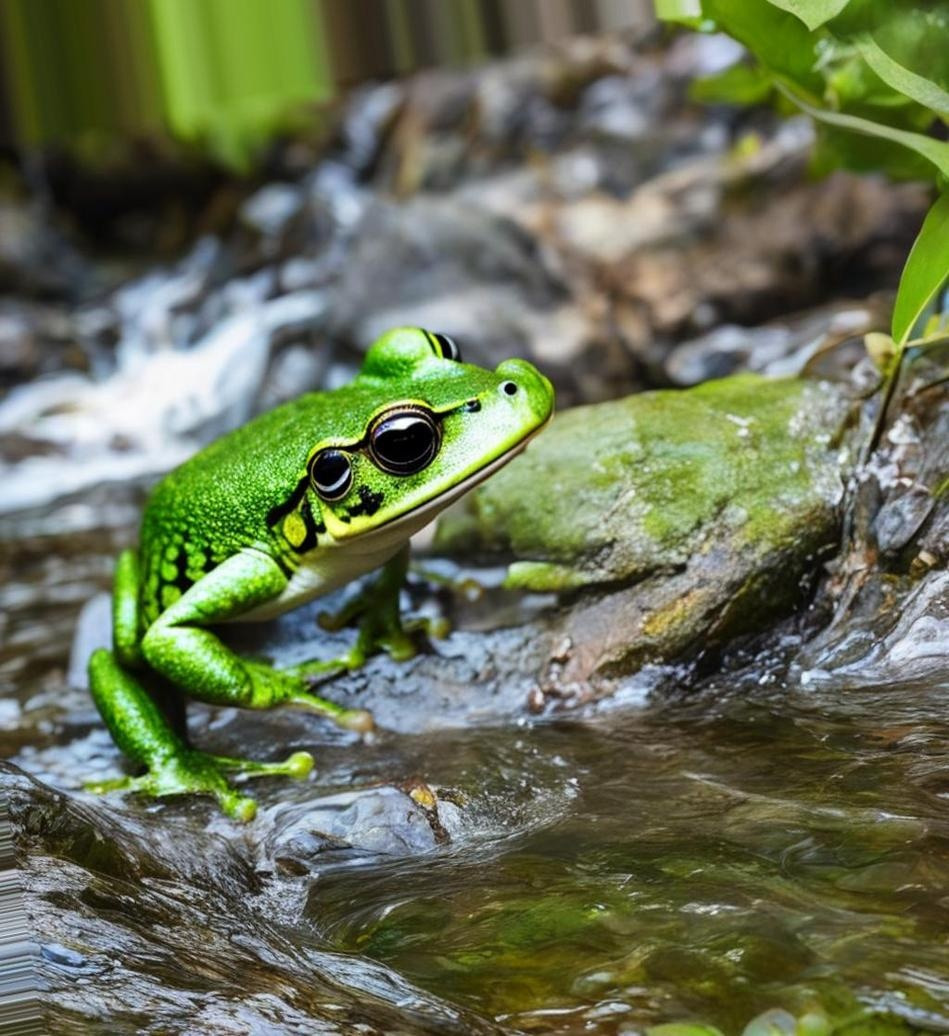
\includegraphics[width=.4\linewidth]{trained_two_classes/negative_imagen_880}
            \caption{Negative class in the training data of the challenge}
            \label{fig:negative-trained_two_classes}
        \end{subfigure}

        \begin{subfigure}{.9\textwidth}
            \centering
            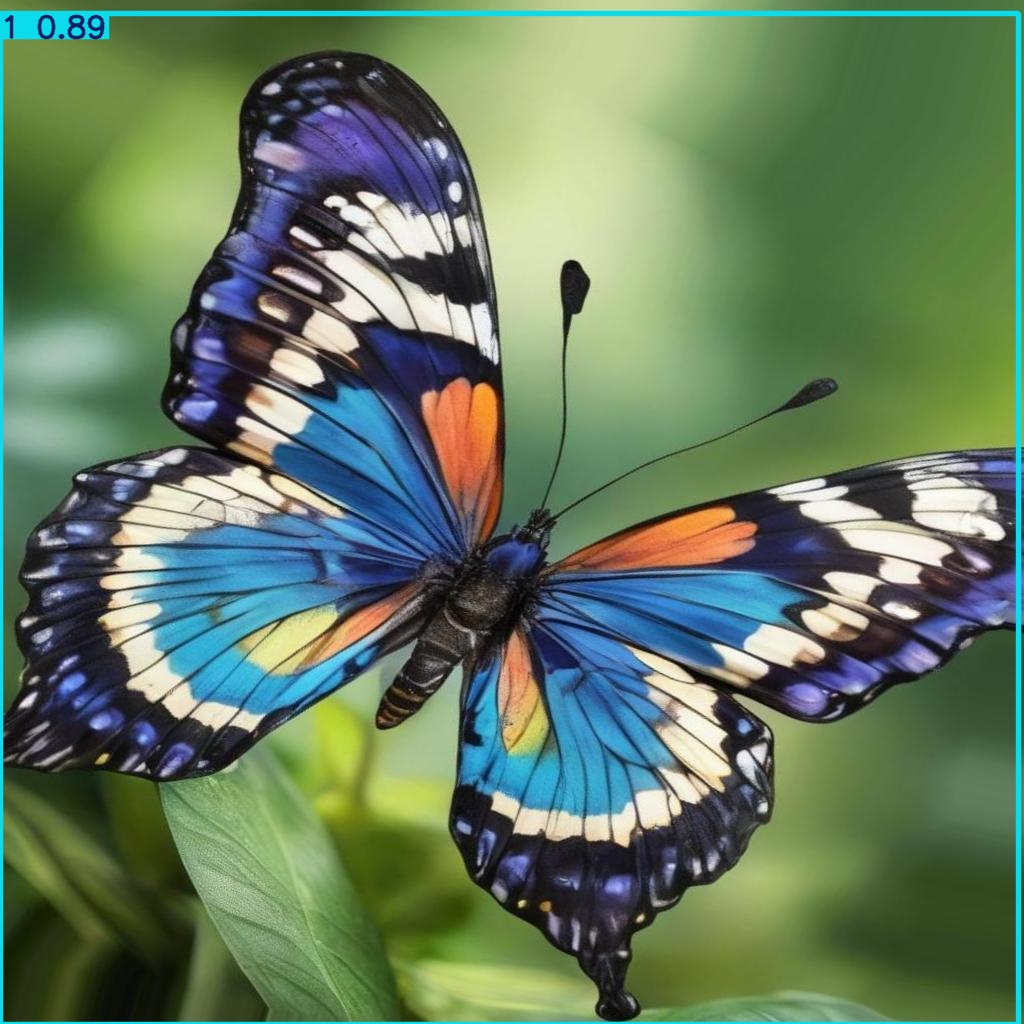
\includegraphics[width=.4\linewidth]{trained_two_classes/positive_imagen_45}
            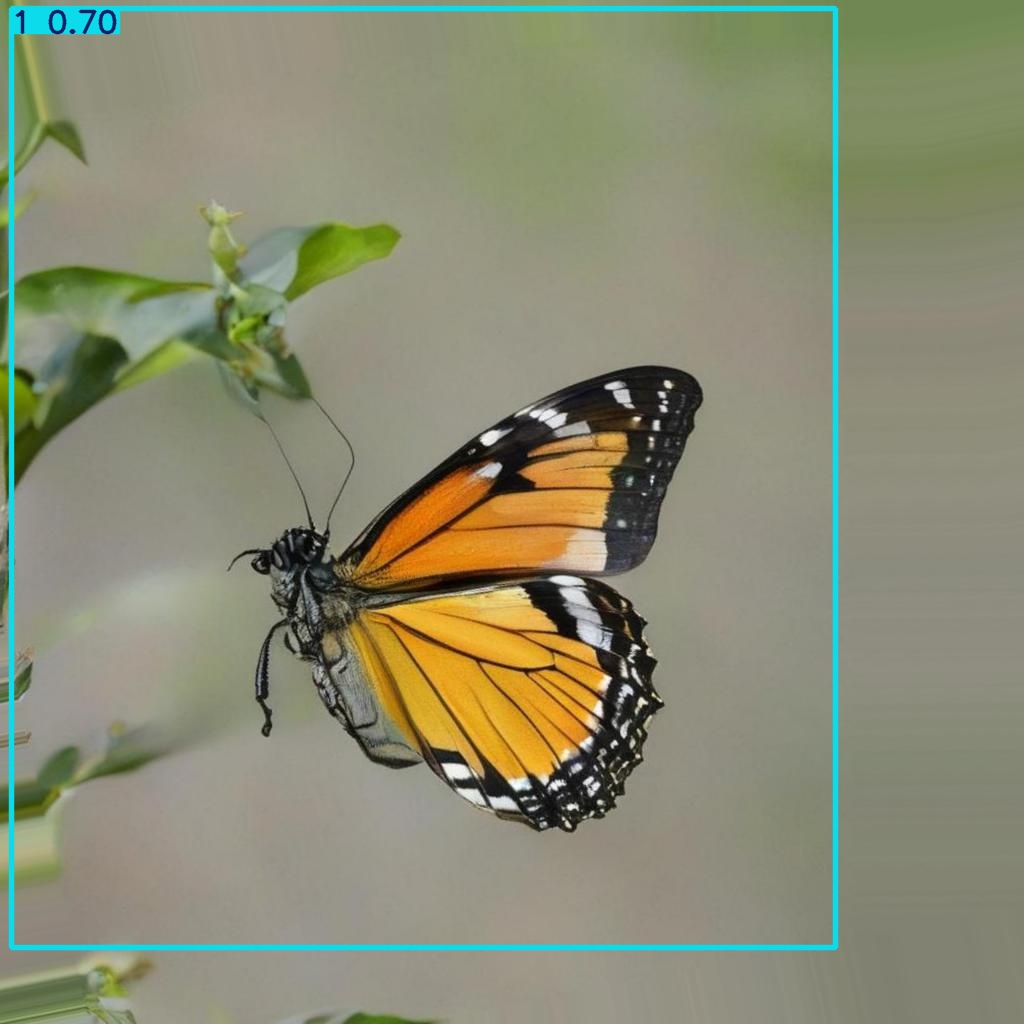
\includegraphics[width=.4\linewidth]{trained_two_classes/positive_imagen_888}
            \caption{Positive class in the training data of the challenge}
            \label{fig:positive-trained_two_classes}
        \end{subfigure}

        \begin{subfigure}{.9\textwidth}
            \centering
            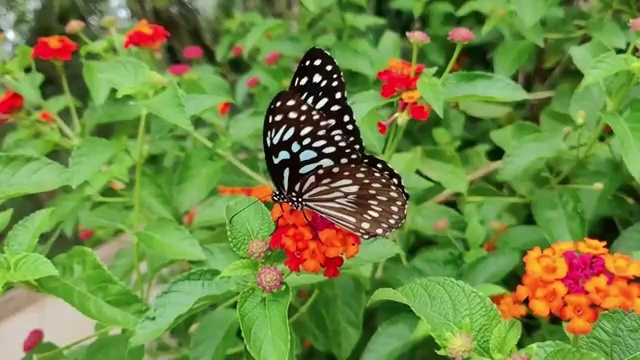
\includegraphics[width=.4\linewidth]{trained_two_classes/photogram_16}
            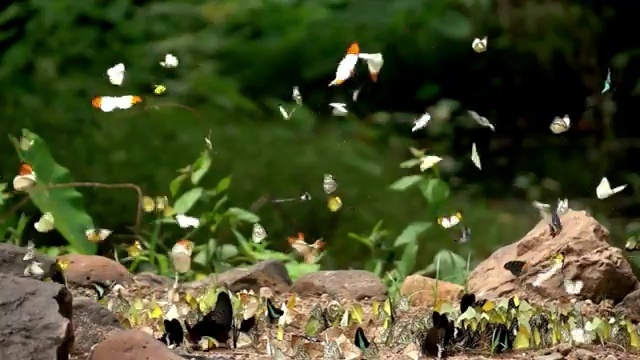
\includegraphics[width=.4\linewidth]{trained_two_classes/photogram_93}
            \caption{Images of the YouTube video}
            \label{fig:video-trained_two_classes}
        \end{subfigure}
        \caption{Images results using transfer learning with just two classes, butterflies and moths}
        \label{fig:trained_two_classes}
    \end{figure}

\end{document}